\documentclass{report}
\usepackage[utf8]{inputenc}
\usepackage{import}
\usepackage[nottoc, notlof, notlot]{tocbibind}
\usepackage{appendix}
\usepackage{hyperref}
\usepackage{graphicx}
\usepackage[backend=biber,style=alphabetic,sorting=ynt]{biblatex}
\usepackage{url}
\usepackage{listings}
\usepackage{minted}
% \usepackage[linesnumbered,ruled,vlined]{algorithm2e}
\usepackage{caption}
\usepackage[acronym, toc]{glossaries}
\usepackage{amsmath} 

\graphicspath{ {./images/} }
\addbibresource{refs.bib}

\setlength{\parindent}{0em}
\setlength{\parskip}{1em}

\title{Offroads: A Trail Running Website}
\author{John Omokhodion Iyere }

\date{April 2019}

\makeglossaries

\newglossaryentry{introspect}{
    name=introspect,
    description={ask the GraphQl schema about what queries it supports}
}

\newglossaryentry{backend}{
    name=backend,
    description={in a client-server web application, the backend refers to the server.}
}

\newglossaryentry{frontend}{
    name=frontend,
    description={in a client-server web application, the frontend refers to the client the user interacts with}
}

\newacronym{rest}{REST}{Representational State Transfer}
\newacronym{orm}{ORM}{Object-relational mapping}
\newacronym{dal}{DAL}{Data Access Layer}
\newacronym{crud}{CRUD}{Create, Read, Update and Delete}
\newacronym{json}{JSON}{Javascript Object Notation}
\newacronym{jwt}{JWT}{JSON Web Token}
\newacronym{hmac}{HMAC}{Hash-based Message Authentication Code}
\newacronym{hs256}{HS356}{HMAC with SHA-256}

\begin{document}

\maketitle
\chapter*{Abstract}
Recommender systems are at the core most modern businesses. It solves the non-trivial problem of keeping high user engagement with a service being provided by ensuring attempting to suggest items to that is both personalised and desired by each specific user. Because of this Recommender systems have become an important and heavily active important area of research, gathering a variety of different algorithms and now more recently, being approached by from the Machine Learning world. This report  explores and exploit the benefits of Recommender systems via a Trail running website. This also proposes the problem of building a highly interactive acutely complex modern web application, one that requires a map interface to offer trail creation capabilities and a view for trail presentation. Hence we also need to examine the various technologies award an expert production.

\chapter*{Acknowledgements}
I would like to thank my supervisor Dr. James Miles for his continued support and guidance throughout the entire life-cycle of this project. Without his advice, this process would have been even more difficult than it already was.

I would also like to express my gratitude to my friends and family for their continued encouragement during the project.

Finally I would like to declare the deepest and greatest appreciation to my mum, for being nonstop strength and cheer-leading that she unrelentingly offered. 
\tableofcontents
\listoffigures
\listoftables
\listoflistings

\newpage

\chapter{Introduction} \label{chap:Intro}
Trail Running is an activity that involves running a path generally stationed in a natural environment such as forested or hilly spaces \cite{wiki:TrailRunning}. It's an activity upheld by a large number of participants and, as with most activities has garnered a community whom require a means of facilitating the creation and discovery of trails within the community. Hence we are presented with three main issues this project aims to resolve:
\begin{itemize}
    \item Provide an interface that buoys astute \textbf{trail creation} as discussed in chapter \ref{chap:TrailInterface}.
    \item Create a \textbf{platform} that encourages sharing and critiquing of these created trails within a community discussed in chapter \ref{chap:Architecture}.
    \item Design a system that cleverly \textbf{recommends} new trails are best suited to a specific user discussed in chapter \ref{chap:Recommender}.
\end{itemize}
This project aims to explore the technologies, methodologies, and algorithms that are best suited to approaching the specification outlined above and delivering the results in the form of a modern web application.


\chapter{Background}
Others have approached the objectives highlighted in \autoref{chap:Intro} in the form of Trail Running Applications, and Recommender systems. Therefore, researching related works and existing solutions is imperative to understanding these topic areas and help advise the approach taken by the project.

\section{Trail Running Applications} \label{sec:TrailRunningApplications}
Many applications provide the functionality to support trail running. They equip the user with an interface that empowers them with tools to create and discover trails via web applications and\\or mobile applications such as Strava. 

\subsubsection{Strava}
Strava is a popular application that provides trail running services to its users with its website and mobile application \cite{strava}.  The primary focus is fitness and competition.  It does this by allowing users to upload \acrfull{gps} data and recorded times of runs they have performed on a trail. These details are used to populate leader-boards and generate rankings on trails.


There are other many other trail running applications such as \acrfull{os} Maps, Mapometer and others. They all provide a Map Interface that allows users to create trails by clicking on points on the map and connecting the points with a line. They include searches, maps, and details on trails to help their users find what type of trail they wish to use. However, they all fail at giving personalised trails to each user. Although they use location information (trails in the user's immediate area), they do not use any information retrieval techniques to get tailored trails to each user, also known as Recommender Systems explained in section \ref{sec:RecSystems}

\begin{figure}[ht]
    \centering
    \includegraphics[width=\textwidth]{images/os-maps-editor.png}
    \caption{OS Maps trail editor that allows user to create trails by clicking on points on the map}
    \label{fig:osMapsEditor}
\end{figure}

\section{Recommender Systems} \label{sec:RecSystems}
Recommender systems are a type of Information Filtering System that provide suggestions personalised to an intended user \cite{ricci2011introduction}.  Recommender systems arose as a solution to the problem of too many options, especially with the age of the Internet where businesses can make available even more products and/or services \cite{rishabh2019recommender}.  By trying to determine each users preferences, the system can suggest items that are appropriate to each specific user.  The term ``item" can refer to almost any product or service that requires a users choice, for trail running, it refers to the trails. We can see  Recommender Systems in most areas such as,  movies,  products, news, people and so on.

\subsection{Why Recommender Systems} \label{subsec:WhyRecSystems}
In 1896, the Italian Economist Vilfredo Pareto proposed a theory that for events, \textit{``80\% of the effects, come from 20\% of the causes" \cite{sanders1987pareto}}. This theory is known as the Pareto Principle and is more commonly know as the 80/20 rule. Traditionally, this rule is a popular maxim in business and strategy management, based on the idea that 80\% of sales can be generated by 20\% of the items being offered, commonly referred to as the ``best selling items".

However, in a 2004 article in \textbf{Wired} Magazine, Chris Anderson observed that on the internet, businesses can be more profitable by offering a larger number of niche, hard-to-find products \cite{brynjolfsson2011goodbye}. This phenomenon was coined \textbf{the Long Tail Effect}, further discussed in Chris Anderson's book \textit{``The Long Tail: Why the Future of Business Is Selling Less of More"} \cite{anderson2006long}. He explains that this new trend is is due to the the improvement in technology that enables users to search and discover more easily. 

\begin{figure}[htb!]
    \centering
    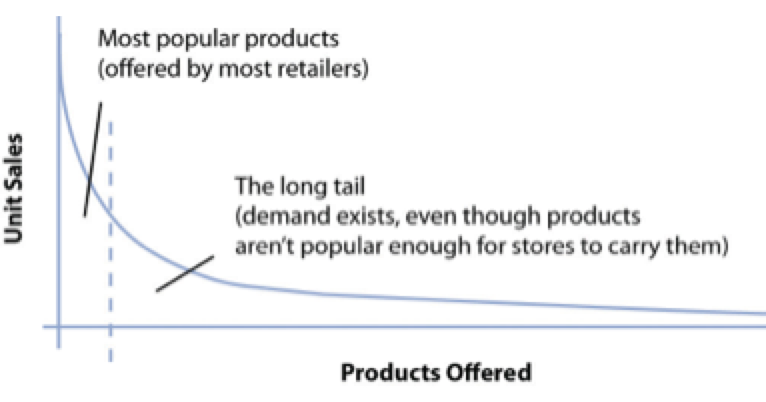
\includegraphics[width=0.75\textwidth]{long-tail.png}
    \caption{The long tail effect \cite{longtaileffect}}
    \label{fig:longtail}
\end{figure}

It especially was strengthened by the advent of Recommender Systems. By offering more personalised items to users, we can expose users to these hard-to-find items that would have been apparent in on a popularity list. Proof of the advantages Recommender Systems offer can be seen by the major companies that take advantage of these systems.


\subsubsection{Amazon} 
Amazon is a behemoth multi-billion dollar online retail company. According to Statista, in 2018, they generated 232.89 billion dollars \cite{statista}. In a 2013 article by Mckinsey \& Company, it is reported that 35\% of Amazon's revenue comes from its recommendation System. 

\subsubsection{Netflix}
Netflix is an online video streaming platform that offers thousands of TV Series and Movies to it's millions of users. Netflix uses a Recommender System not only to personalise the videos offered to the user, but also the artwork that is used as the thumbnail\footnote{a cover image for a video} for the video \cite{josefina2018netflix}.

These are just a few examples of platforms that benefit from Recommender systems \cite{polatidis2013recommender}.

\subsection{Machine Learning Approach} \label{subsec:mlApproach}
Machine Learning is a study of Artificial Intelligence that uses algorithms and models to enable computer systems learn how to perform tasks using data without the need for explicit instructions to be given \cite{michie1994machine}. Machine learning models are used for a variety of tasks such as classification\footnote{differentiation between items}, facial recognition, regression analysis and so on.

Regression Analysis is a set of techniques that discover relationships between variables in data \cite{chatterjee2015regression}. By trying to find a best fit between variables in data, you can discover the relationship between them and also predict values for new variables. Regression analysis can also be described as a predictive analysis, hence, Recommender Systems can be classified as a Regression Analysis problem, as the system try's to predict a user's predicted rating of an Item. Hence we have a means to creating a Recommender System using Machine learning Methods.

\section{GraphQL over REST}
Web applications consists of two main parts: the client, which contains the user interface the user interacts with, and the server, which provides the resources needed to be consumed by the client. In recent years, \acrfull{rest} has quickly been adopted in industry as the standard for creating a server \acrfull{api} \cite{guy2015rest}. They allow the client to access the resources provided in the server via stateless operations with the use of a \acrfull{url}. However one of the main problems with \acrshort{rest} is it's lack of flexibility. The resources in \acrshort{rest} are exposed via endpoints. The shape of the data returned to the client by theses endpoints are defined by the server. This can lead to problems of \gls{over-fetching} and \gls{under-fetching}. In \autoref{fig:restProblem}, we can see a standard \acrshort{rest} \acrshort{api} that exposes a users details, posts and followers via separate endpoints. The client is forced to make multiple requests to get the data required as each endpoint returns under-fetched. If the client requests only a users name from the user details endpoint, this leads to over-fetching of data.

\begin{figure}[htb!]
    \centering
    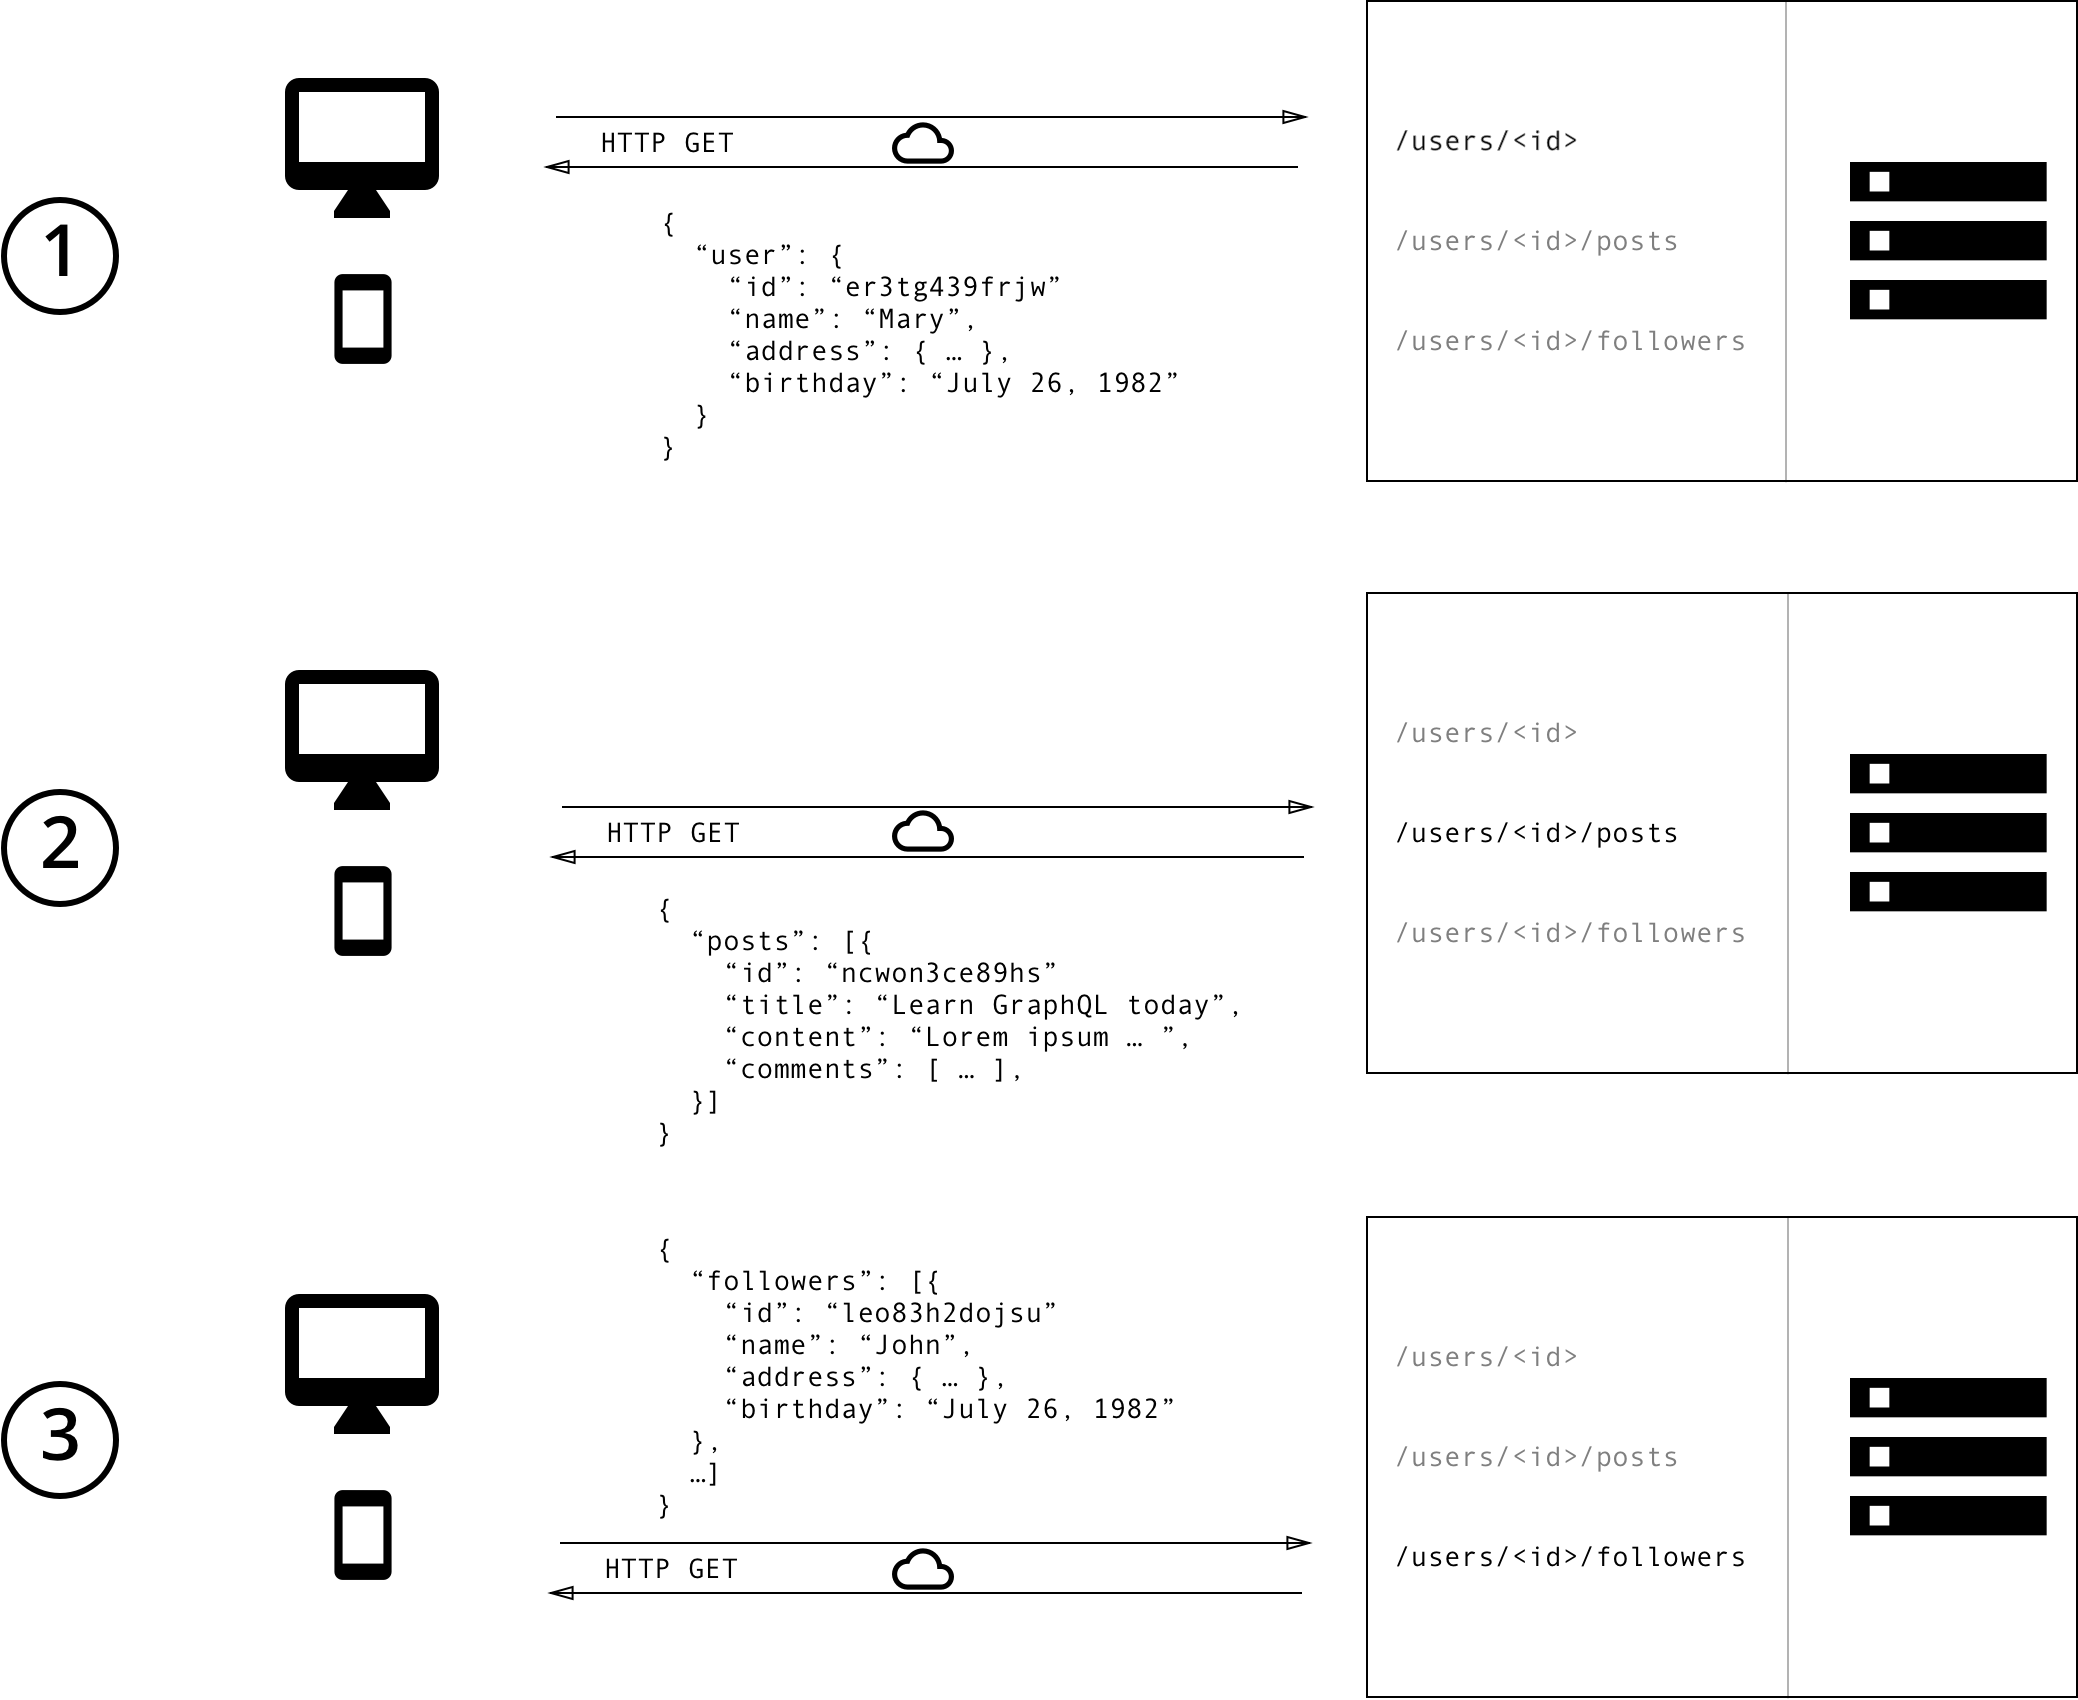
\includegraphics[width=0.75\textwidth]{problems-with-rest.png}
    \caption{REST having to make three separate requests to to three different endpoints to get the required data \cite{graphqlvsRest}}
    \label{fig:restProblem}
\end{figure}

GraphQL was introduced as a solution to the shortcomings with \acrshort{rest} GraphQL, created by Facebook in 2012, and then open sourced in 2015, is a query language for an \acrfull{api} and a run-time for fulfilling those queries with your existing data \cite{graphQl}.  Like \acrshort{rest}, GraphQL is used to expose resources to the client. However, GraphQl only exposes a single endpoint and the client defines the structure of the data that is required \cite{howToGraphQl}, eliminating the problem of over-fetching and over fetching. \autoref{fig:graphqlFix} shows how a GraphQL server can get the same data as the before, using only one request.

\begin{figure}[htb!]
    \centering
    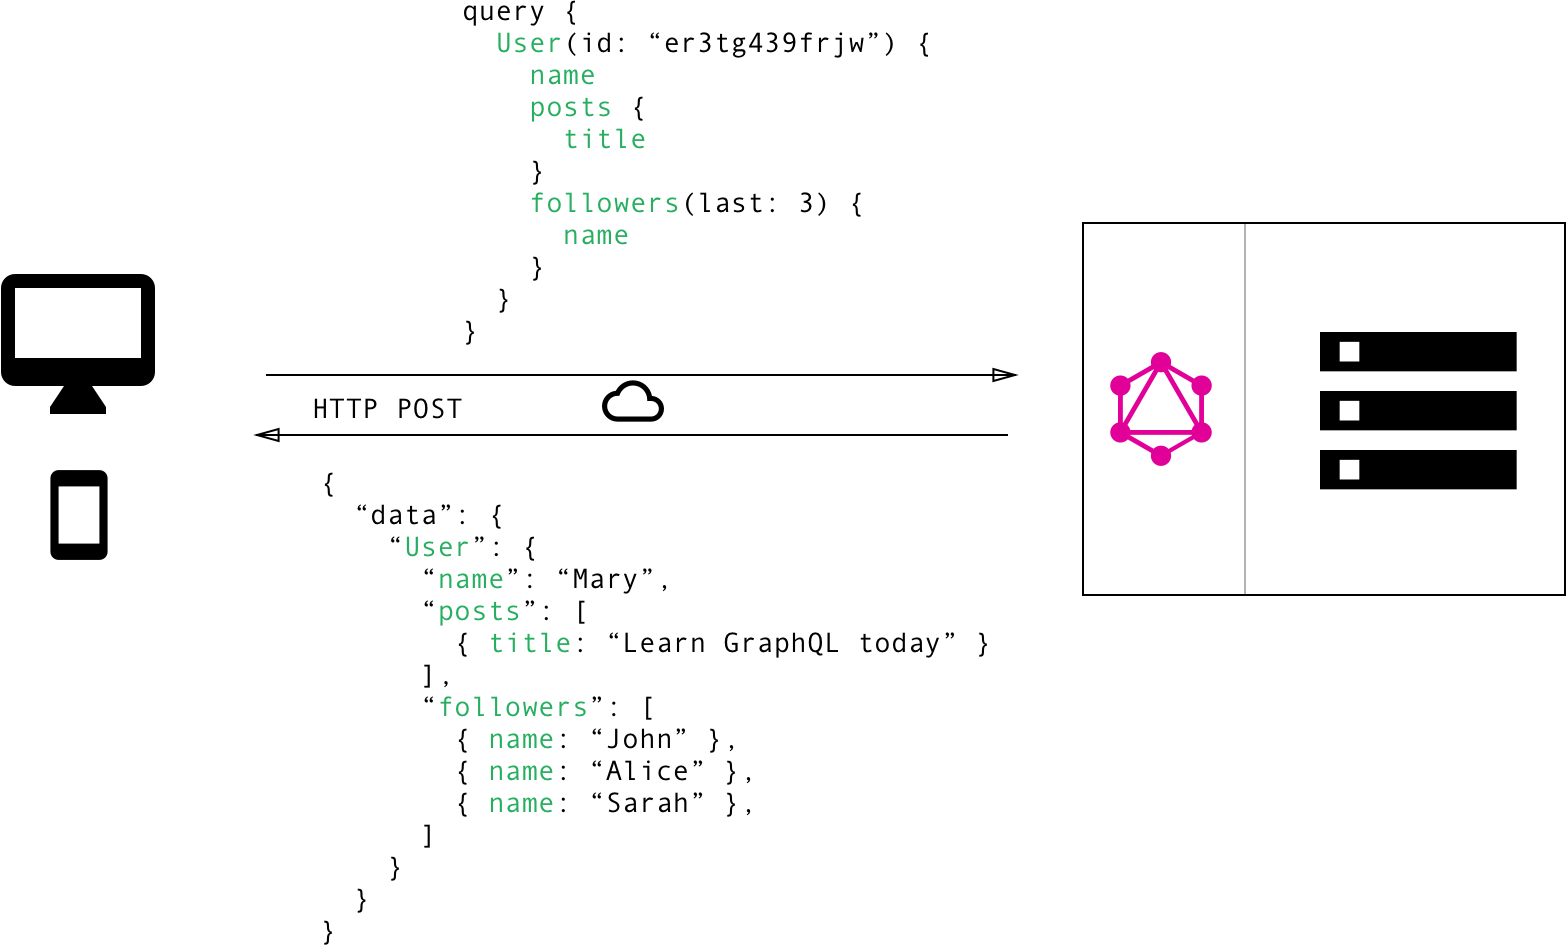
\includegraphics[width=0.75\textwidth]{fetching-graphql.png}
    \caption{GraphQl can perform retrieve the same required data using one request to one endpoint \cite{graphqlSolution}}
    \label{fig:graphqlFix}
\end{figure}

This is important in our application as in some scenarios where information is being retrieved, we would want to prevent over-fetching. To store trail information, a large number of coordinates per each trail needs to be stored. When a user is searching for a trail initially, only details such as the name of the trail, average rating and so on are required. Requesting all the coordinates would add unnecessary overhead to the system during communication between the client and server.
\chapter{An Interface For Trails} \label{chap:TrailInterface}
To facilitate the creation and exhibition of trails on a website, it is important to provide and interface that assists in bring visual and contextual aid to the users as they are planning a path or exploring other paths. This chapter describes the two main methods used to provide such information via a Map Interface (discussed in section \ref{mappingPlatform}), and an Elevation Profile (discussed in section \ref{elevationProfile}. We discuss the decisions made and technologies used to provide these features.

\section{Mapping Platforms Providers} \label{mappingPlatform}
The platform provides an interactive map interface that users use to create trails. Trails are created by users clicking on points on the map. The system then calculates path between each two points created and connects to ensure that trails stay on the defined paths on the map.

To provide this, we need to use an open source map provider for the interface. In industry, there are really three main providers: Google Maps, Mapbox and Ordinance Survey Maps. To decide on what provider to use, I compare the benefits and negatives of all three in table \ref{tab:MappingPlatformsComparison}.
\begin{table}[]
    \centering
    \begin{tabular}{lll}
        \hline
        \multicolumn{1}{c}{Map Provider} & \multicolumn{1}{c}{Advantages} & \multicolumn{1}{c}{Disadvantages} \\ 
        \hline
        \hline
        Google Maps & \begin{tabular}[c]{@{}l@{}}Very Accurate Map\\ Open Source Software\end{tabular} & Not very customizable \\
        \hline
        Mapbox & \begin{tabular}[c]{@{}l@{}}Open source software\\ Very customizable\\ Big community\\ Good documentation\end{tabular} &  \\
        \hline
        OS Maps & Maps are the most detailed & \begin{tabular}[c]{@{}l@{}}Not opened source\\ Only has UK map\end{tabular} \\ 
        \hline
    \end{tabular}
    \caption{Comparison of the different mapping providers that I could use}
    \label{tab:MappingPlatformsComparison}
\end{table}

From the table \ref{tab:MappingPlatformsComparison} above I decided to use Mapbox. The main reasons are due to it's big community and good documentation. These benefits would allow me to more work with the map provider as I would have a wealth of help for issues that appear during development.

\subsection{Creating a Trail}
When a user clicks on the map, the system returns the coordinates of the point the user clicks on the map as shown in listing \ref{listing:exampleCoordinates}.

\begin{listing}[ht]
\caption{Example of coordinates returned from mapbox}
\inputminted[frame=lines,framesep=2mm,baselinestretch=1.2,fontsize=\footnotesize]{json}{listings/example-coordinates.json}
\label{listing:exampleCoordinates}
\end{listing}

We can use this data to draw points on the map interface, visually showing the user the points that have been clicked as shown in figure \ref{fig:SinglePointCreated}. 
\begin{figure}[ht]
    \centering
    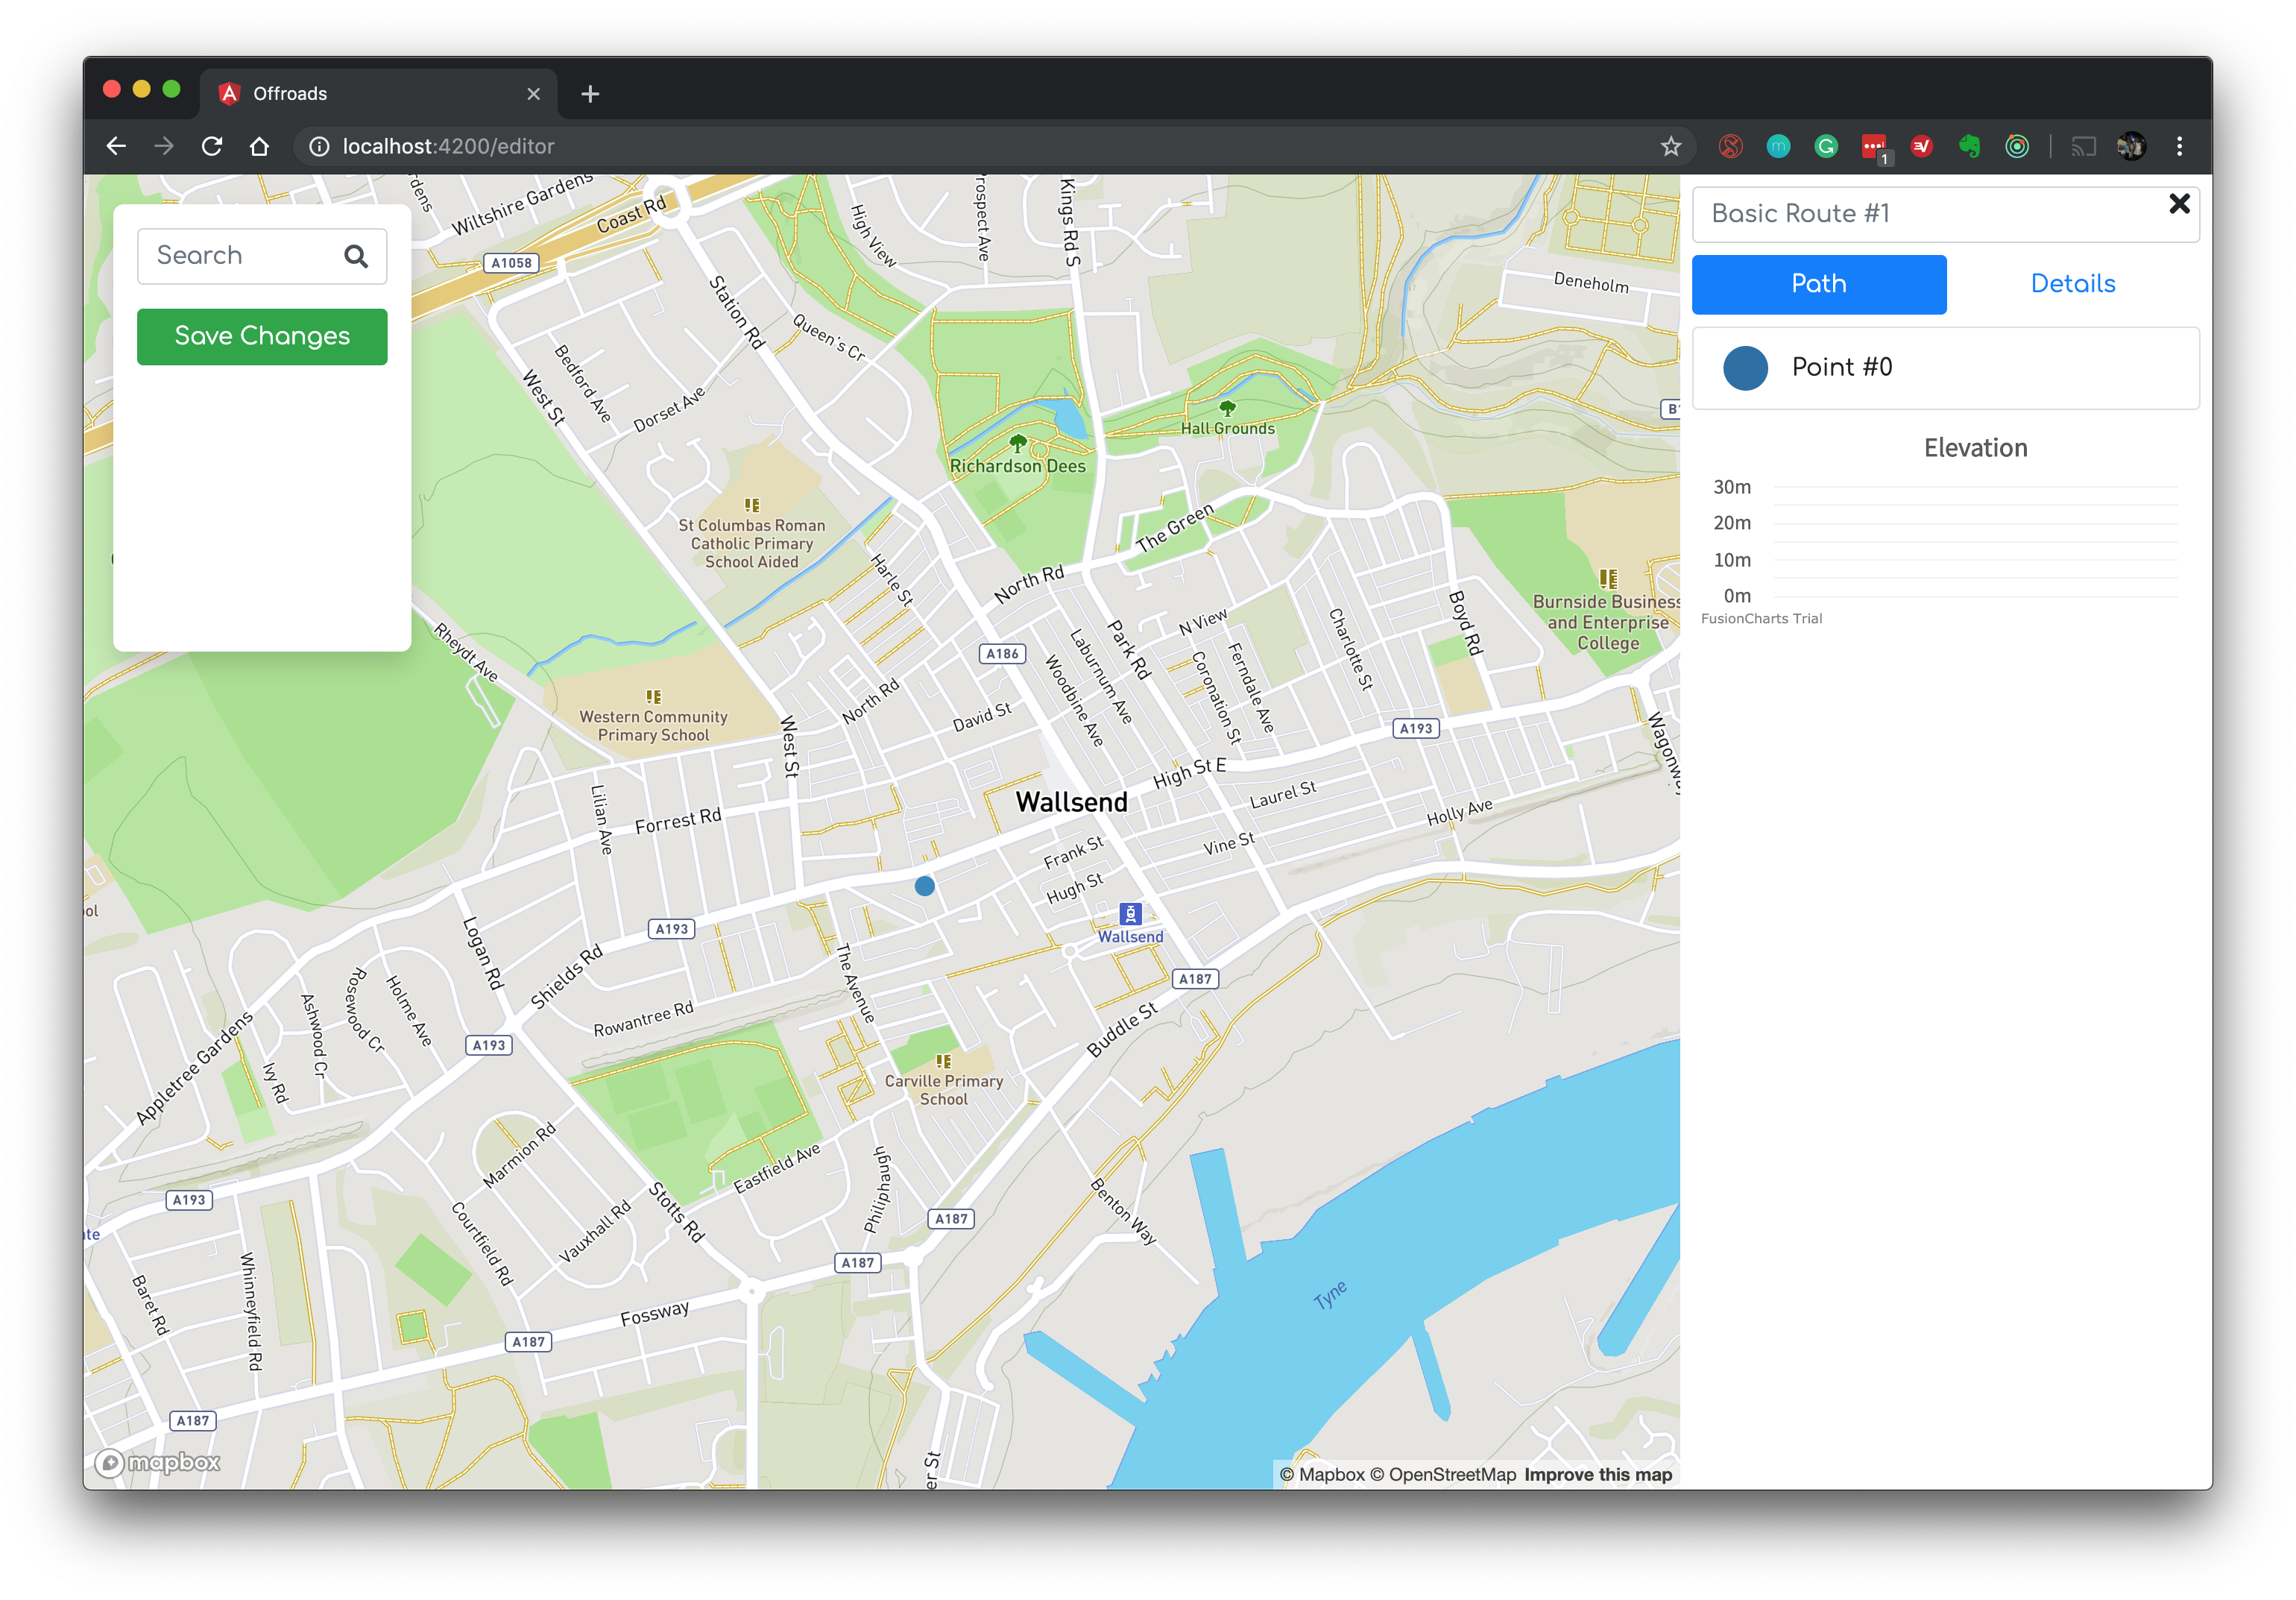
\includegraphics[width=0.75\textwidth]{single-point-on-map.png}
    \caption{The point created by a user clicking on the map indicating the location the user clicked in}
    \label{fig:SinglePointCreated}
\end{figure}
When the user adds an extra point, the system needs to combine these two points with a line. At this point, we need to calculate a path between the last point added and the new point that's just been added. When a user creates a path, it makes more sense for the path to follow already existing paths rather than just a straight line. Hence we need to calculate a path from between the two points to draw the line. Mapbox provides a Directions API to help us do this.


\subsubsection{Finding a path}
Mapbox's Direction API allows us to find a path between two points by querying the API with a \textit{start} and \textit{end} coordinates.  The API then returns us a a json object describing the path between the specified starts and end points and the distance between the two points specified (an example is shown in appendix \ref{appSec:mapboxDirections}). We we use this data to draw a line between the two points that will follow the path returned (see figure \ref{fig:PathCreated}).

\begin{figure}[htb!]
    \centering
    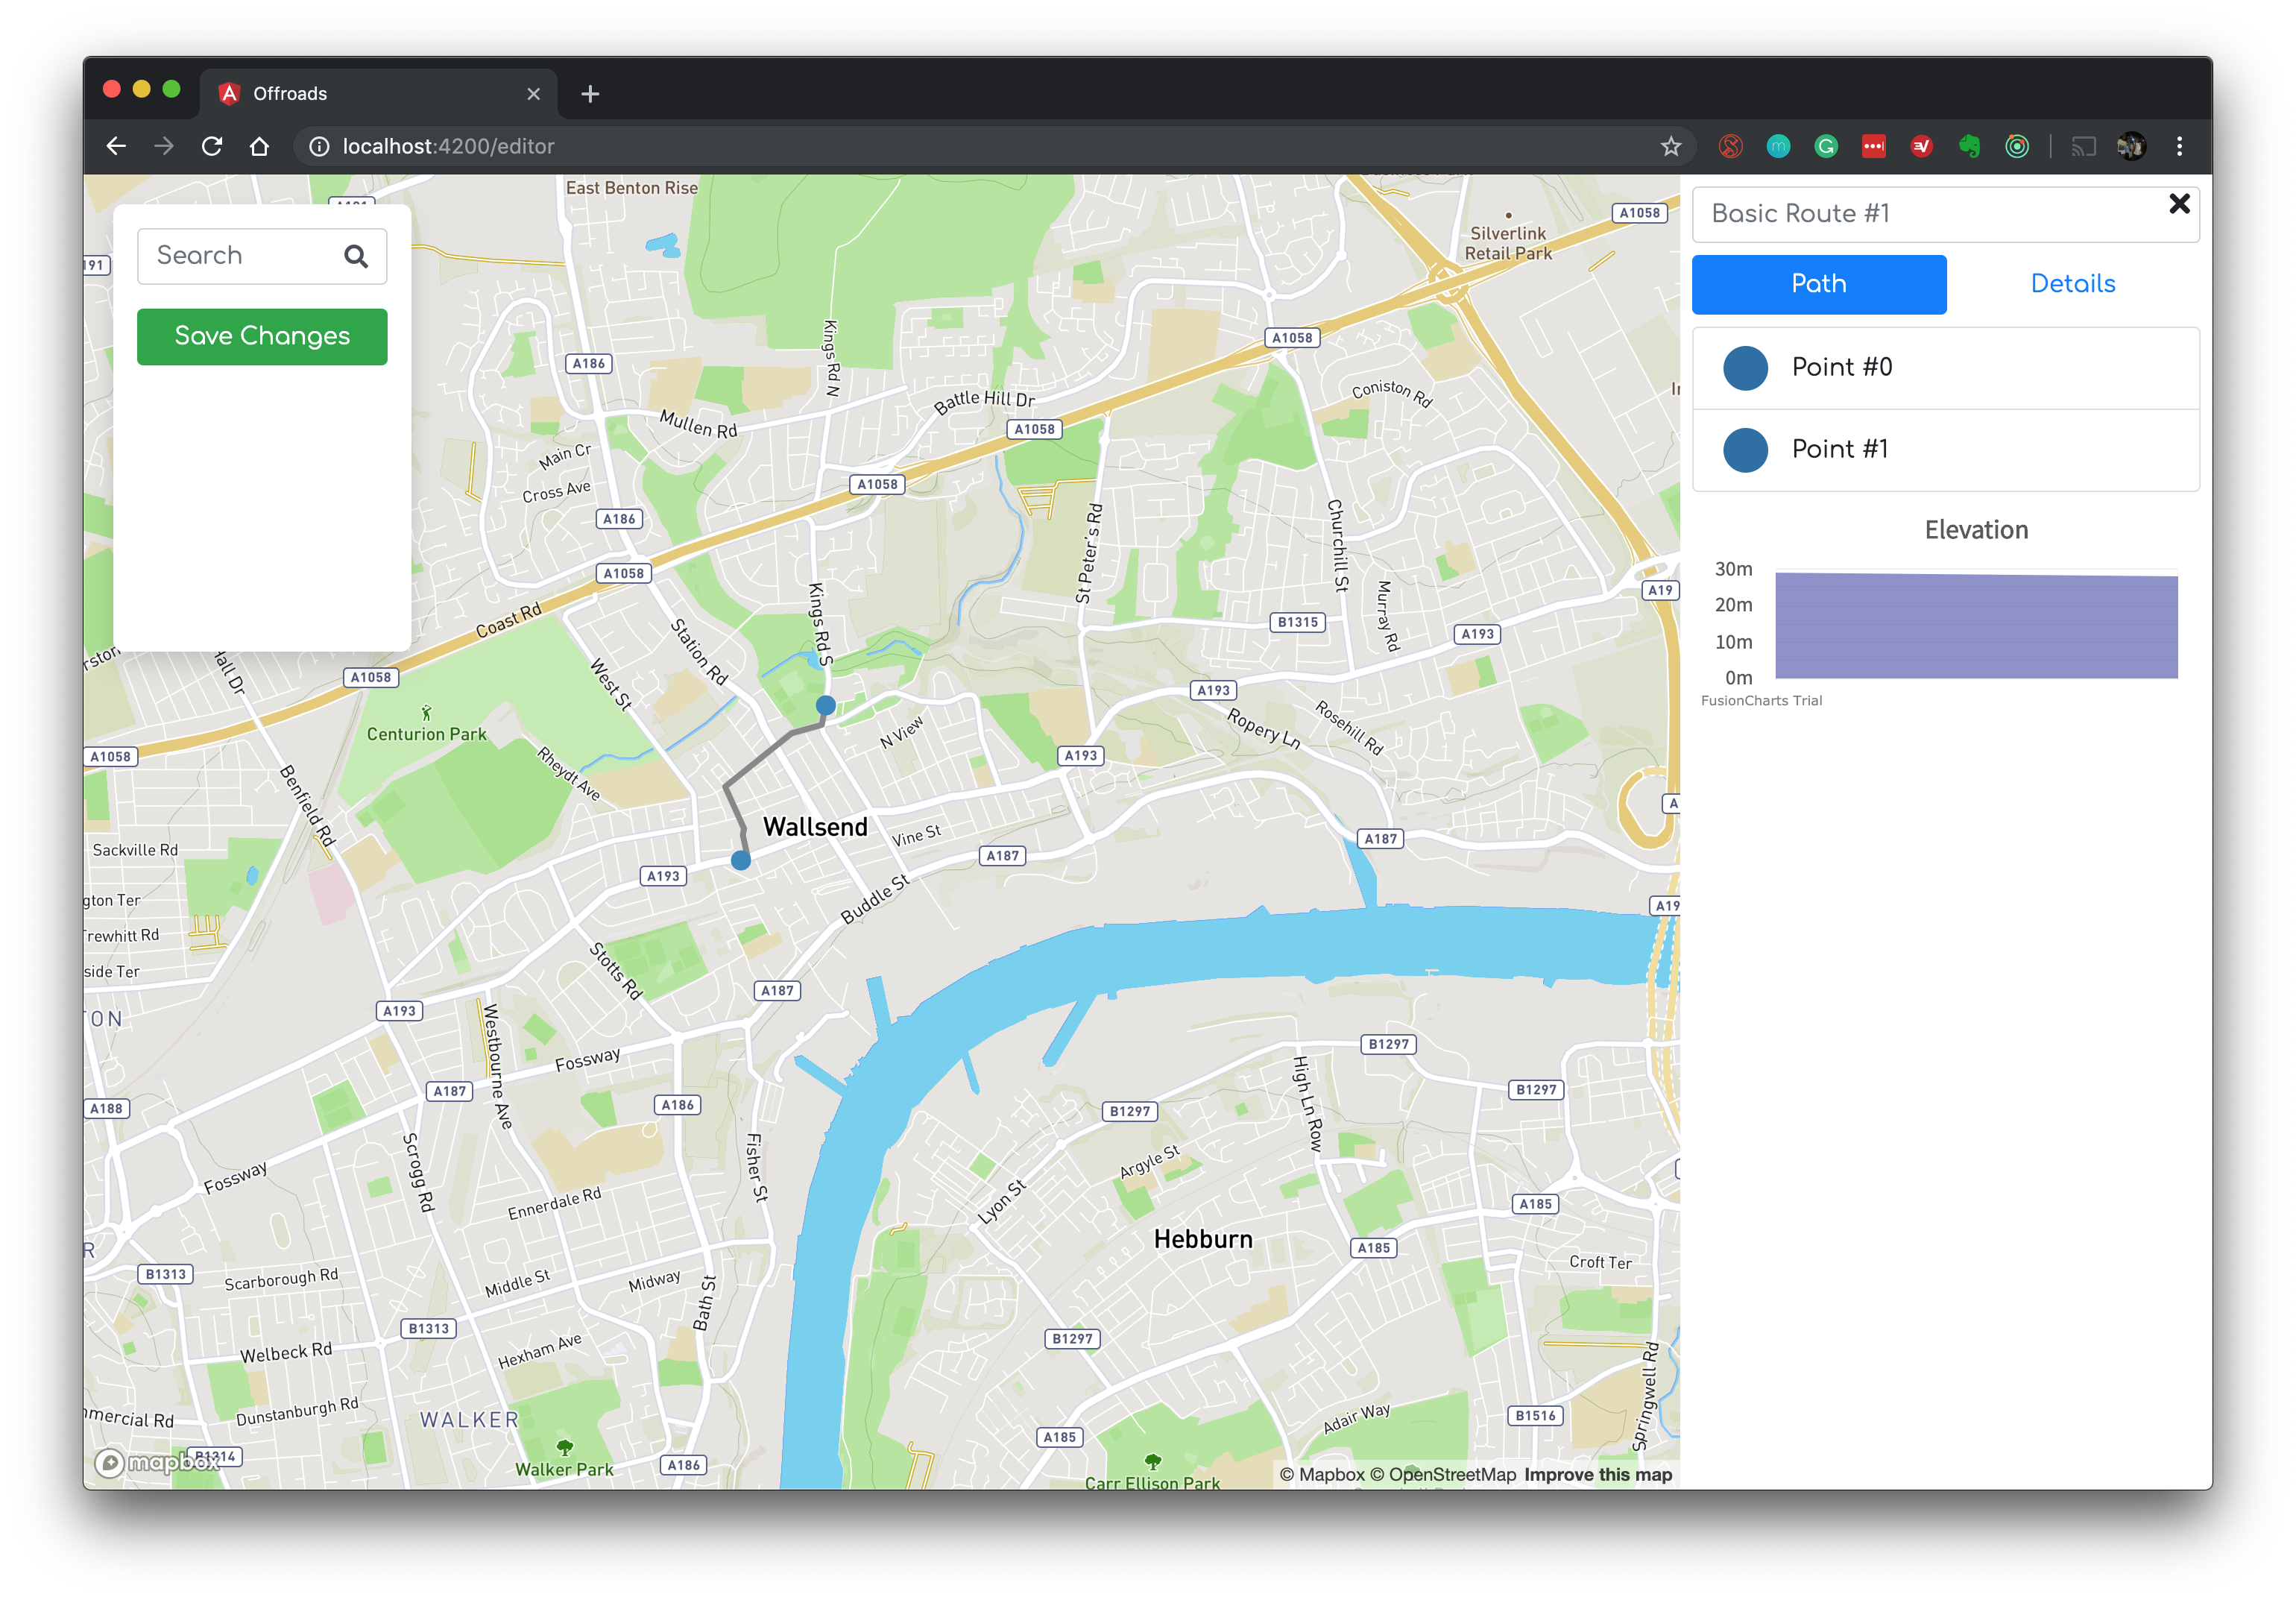
\includegraphics[width=0.75\textwidth]{path-between-points.png}
    \caption{Path created from the directions returned by the Mapbox API}
    \label{fig:PathCreated}
\end{figure}

\section{Presenting Elevation Profiles} \label{elevationProfile}
Trail runner's often use the elevation of a trail to help decide the type of trail that they wish to run. For this, the map interface provides contours that allow users to anticipate the steepness of the trail that they are creating or that they wish to run as shown in figure \ref{fig:MapContours}.

\begin{figure}[htb!]
    \centering
    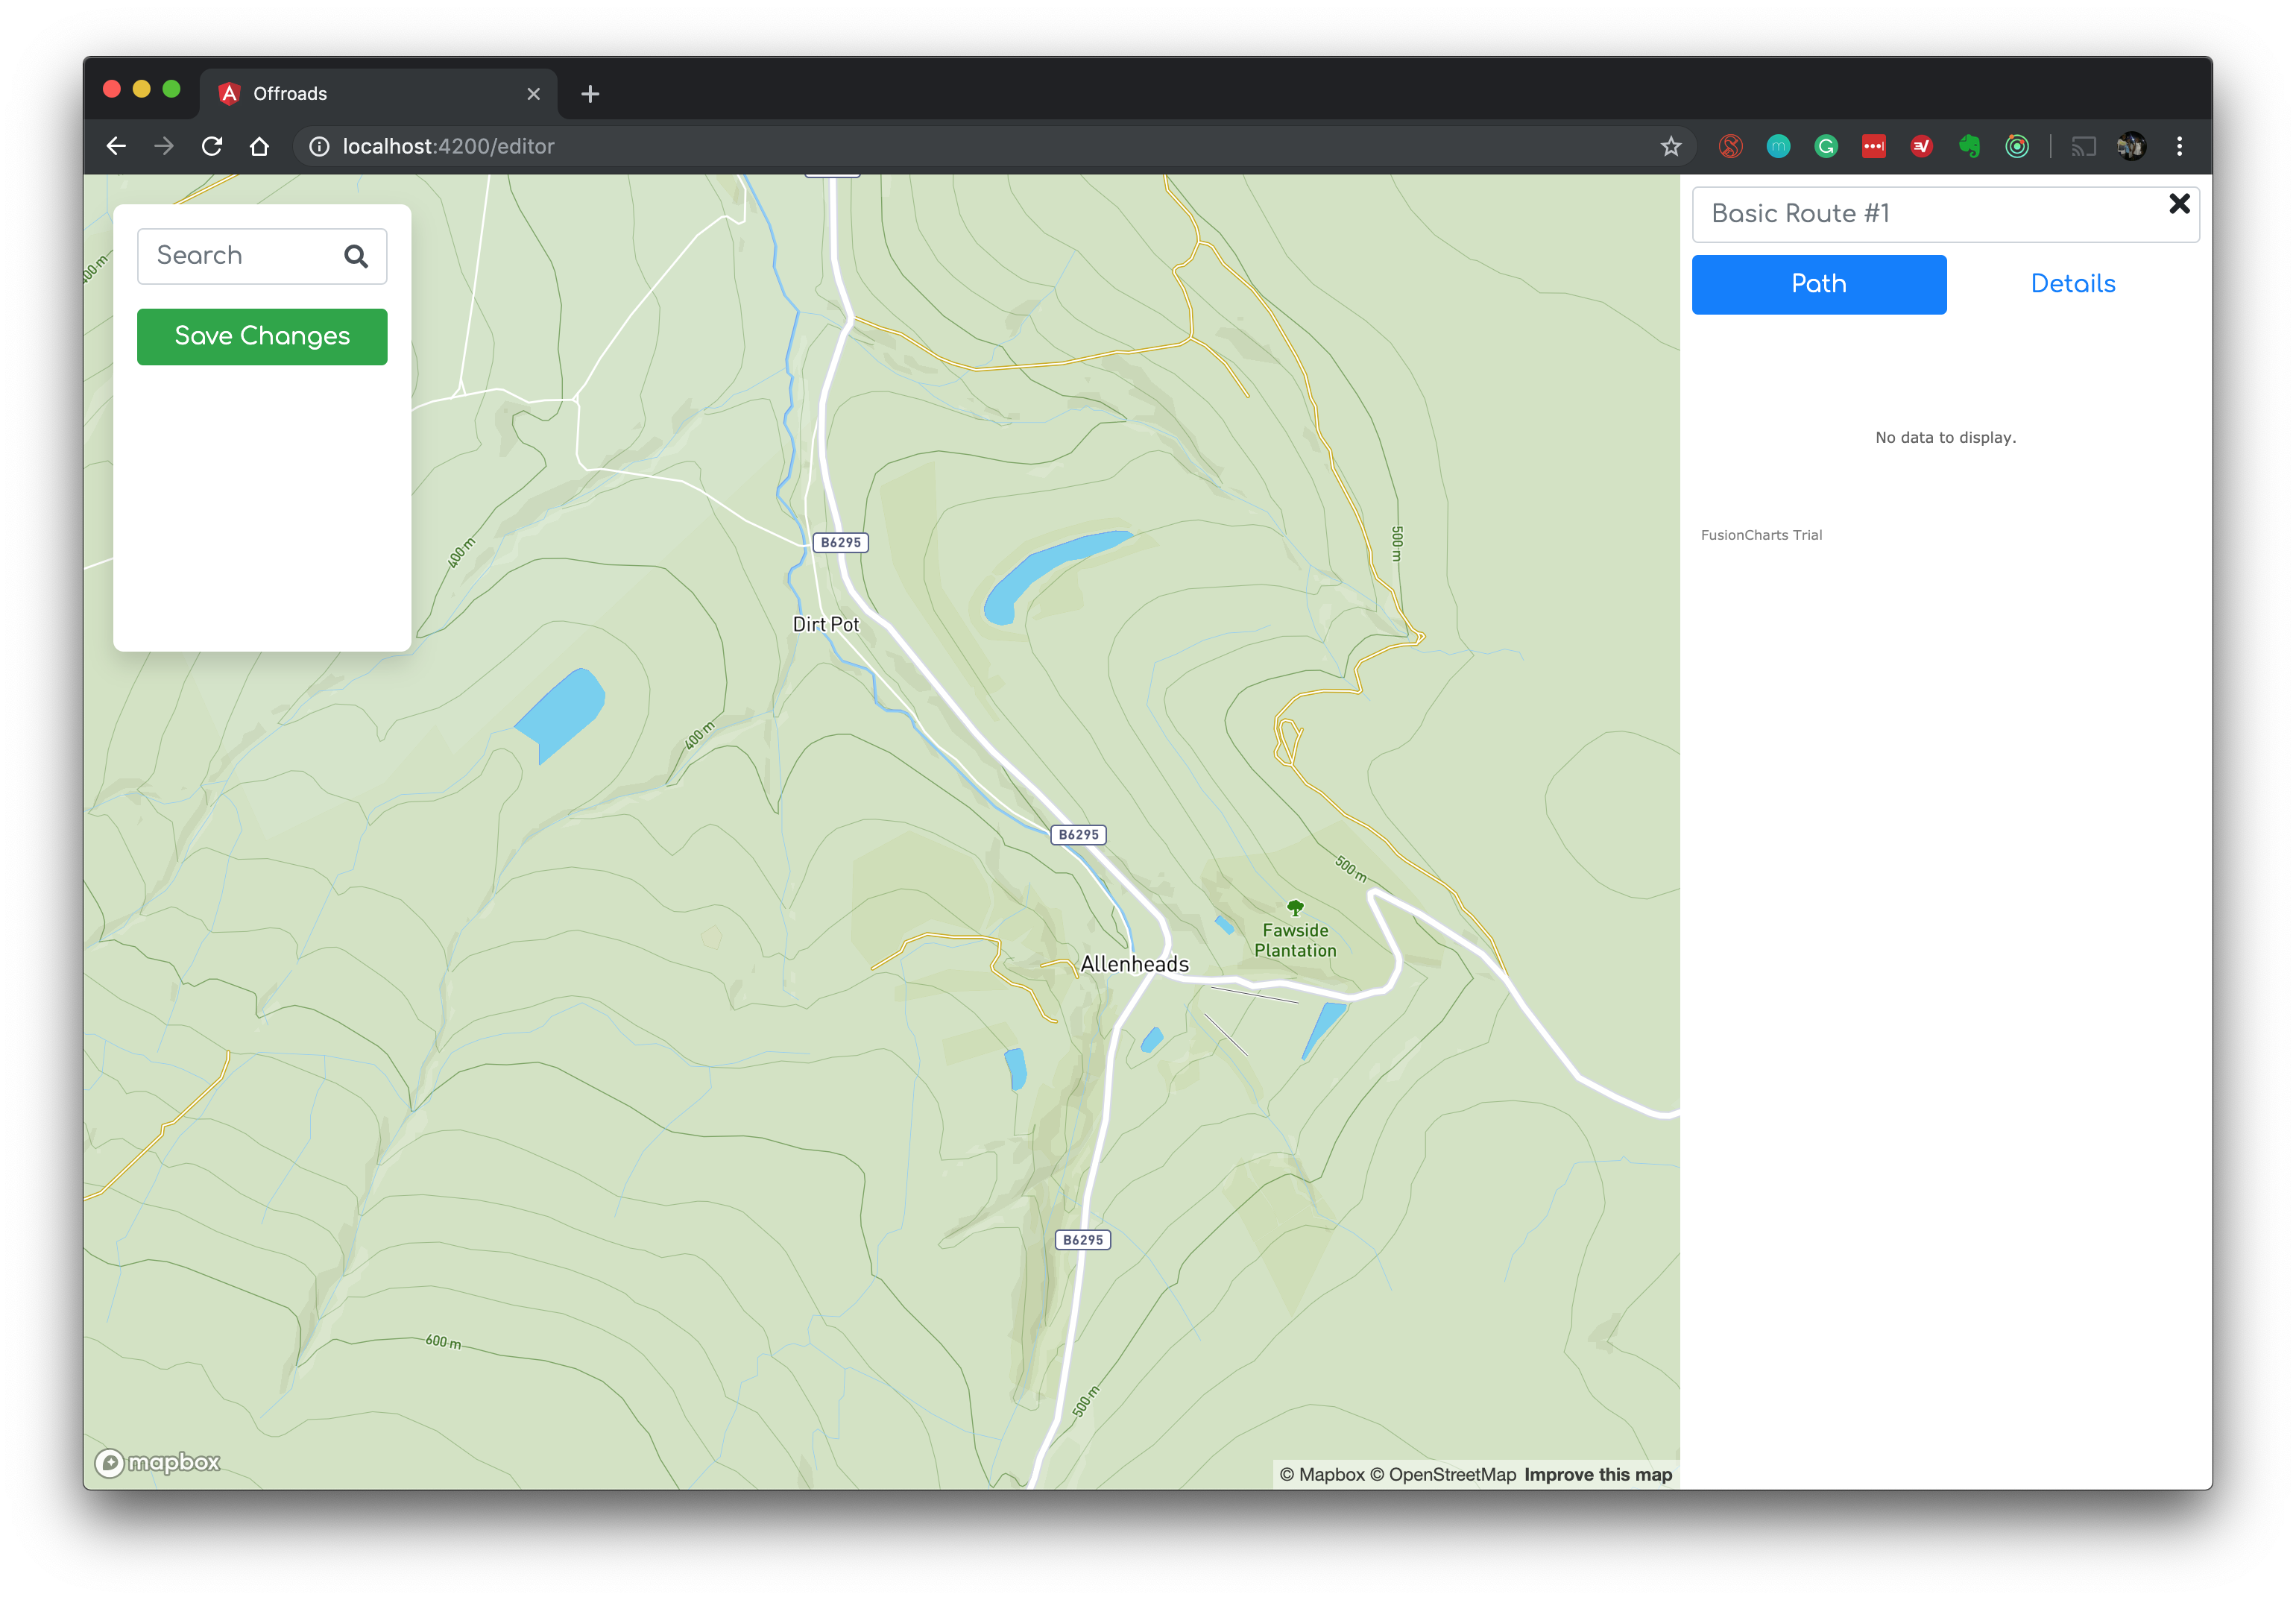
\includegraphics[width=0.75\textwidth]{map-contours.png}
    \caption{Contours on the map to help find elevation}
    \label{fig:MapContours}
\end{figure}


However, for the uninformed, reading contours can prove to be an unusual task. A better way of representing the elevation profile of is via a Graph. This will allow the user to view the elevation of a route against the distance of the route, giving a more detailed view of the elevation of the trail.

The Mapbox Directions API only provides an elevation of specific way-points of the path that is returned as shown in appendix \ref{appSec:mapboxDirections}. Although this provides some elevation information, it is not sufficient enough as the elevation of a trail can change drastically withing way-points.

Google offers an elevation service that allows you to query a specific route and in return get the a detailed elevation of that trail as shown in appendix \ref{appSec:googleElevation}. As a trail is being created, we send another request to the Google elevations service to get this information. We then plot on the graph the line the line that is returned, updating it as we trail is updated. The graphing API that we use is Fusion Charts\cite{fusionCharts}.
\chapter{Architecture} \label{chap:Architecture}
To build Offroads, many technologies needed to be harnessed in order to produce the features needed for the Trail Running Website. In \autoref{chap:TrailInterface} we discussed the interface used to create and display trails, in this chapter we discuss how we provide this interface to the user with our chosen \Gls{frontend} framework in \autoref{sec:frontendFramework}. We discuss the extra features needed that the web application provides in \autoref{sec:ExtraFeatures}.

\section{Overview}
The client of the web application (including the trail interface described in chapter \ref{chap:TrailInterface}) are created with Angular. The client sends to and retrieves data from a GraphQl Server. The GraphQl Server is connected to a MySQl database. Prisma provides a GraphQl \acrfull{dal} to simplify access to the data stored in the database. This overall structure can be seen in \autoref{fig:graphArchitecture}.

\begin{figure}[ht]
    \centering
    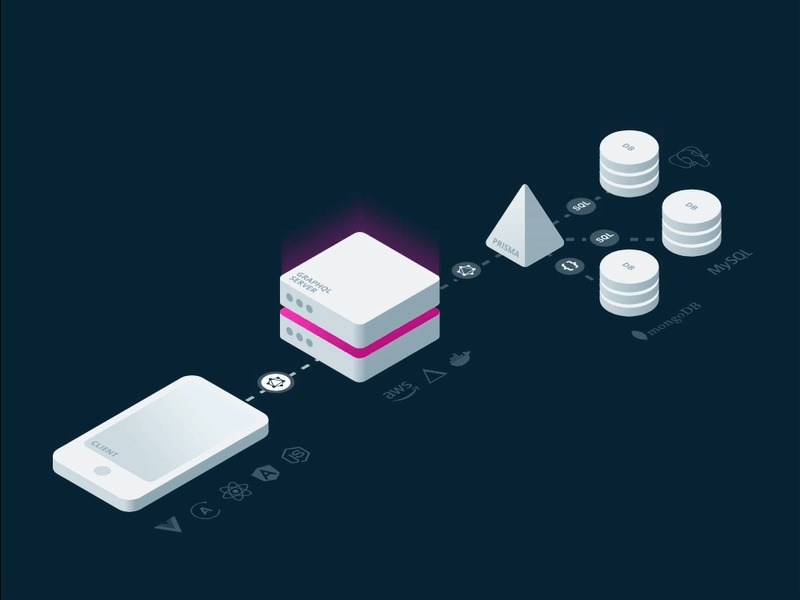
\includegraphics[width=\textwidth]{graphql-architecture.jpg}
    \caption{Overall Architecture of the web application}
    \label{fig:graphArchitecture}
\end{figure}

Our server responds with data written in \acrfull{json} format.

\section{GraphQL Backend}

\subsection{}

\subsection{Prisma Layer}
Prisma\footnote{\url{https://www.prisma.io/}} is a data access layer that replaces traditional ORM's\footnote{Object Relational Mappings}. It sits in front of databases and provides methods that allow the server to access the database. The main feature that it provides is the Prisma Client, which is an auto-generated type-safe database client that creates the data access layer.

\section{Frontend Framework} \label{sec:frontendFramework}
There are 2 main way's to build modern web applications. It can be done using native web stack of HTML, CSS and JavaScript or (and more popularly), built using modern web application frameworks. Although there are many proponents to building with the native web stack, modern applications, such as this one, are more complex in nature and hence, require tools make it easier to build complex solutions. They also have big communities and strong documentation that make debugging easier \cite{medium:WhyModernJSFrameworkExist}.

There are a large variety Frontend Frameworks out there. I considered the most popular ones which where
\begin{itemize}
    \item Angular \footnote{\url{https://angular.io/}}
    \item React \footnote{\url{https://reactjs.org/}}
    \item Vue.js \footnote{\url{https://vuejs.org/}}
\end{itemize}

The framework I decided on was Angular. This was because it has excellent and well-detailed documentation, it came out of the bag with all most of the tools I needed to get started with, and it used Typescript over JavaScript.

Typescript \footnote{\url{https://www.typescriptlang.org/}} is a super set \footnote{it is built on top of JavaScript} of JavaScript, created by Microsoft that provides optional but strict type checking, making developing large scale applications easier \cite{bierman2014understanding}. It also allows me to combine JavaScript's functional programming paradigm \cite{hughes1989functional}, with an Object oriented programming paradigm.

\subsection{State Management With Redux}
One of the main problems that comes with building web applications is managing state in the frontend. On the editor page, where user's create and trails, It is important to manage the state of the application to allow users to undo and redo any changes they make when creating or editing Trails.

It is possible to create your own system to manage state in angular using systems such as Angular's Dependency Injection \cite{wiki:DependencyInjection}, however this does not suffice to handle applications with many interactions. It also doesn't provide standard support for recording user interactions and a means of replaying those steps when needed.

Redux is JavaScript library created by Facebook use for managing state in user interfaces \cite{wiki:Redux}. NgRx \cite{cheng2018state} is a framework built on the fundamentals of Redux\footnote{The Flux Architecture}, to enable us to maintain state in our Application. It is provides a functional way of building Reactive Applications.

With NgRx we can easily manage and control the state of our web application. This is especially useful in on the editor page, where users can create trails described in \autoref{chap:TrailInterface}. With NgRx, we can easily provide undo and redo features. It is common for users to make mistakes when creating a trail, hence allowing users to undo and redo actions they've performed would be hugely beneficial. NgRx helps us manage the state tree (shown in \autoref{fig:reduxStateTree}) of our application in the form of a stack, including the actions users use to create trails. This allows us to traverse the stack of the users actions allowing for redoing and undoing.

\begin{figure}[htb!]
    \centering
    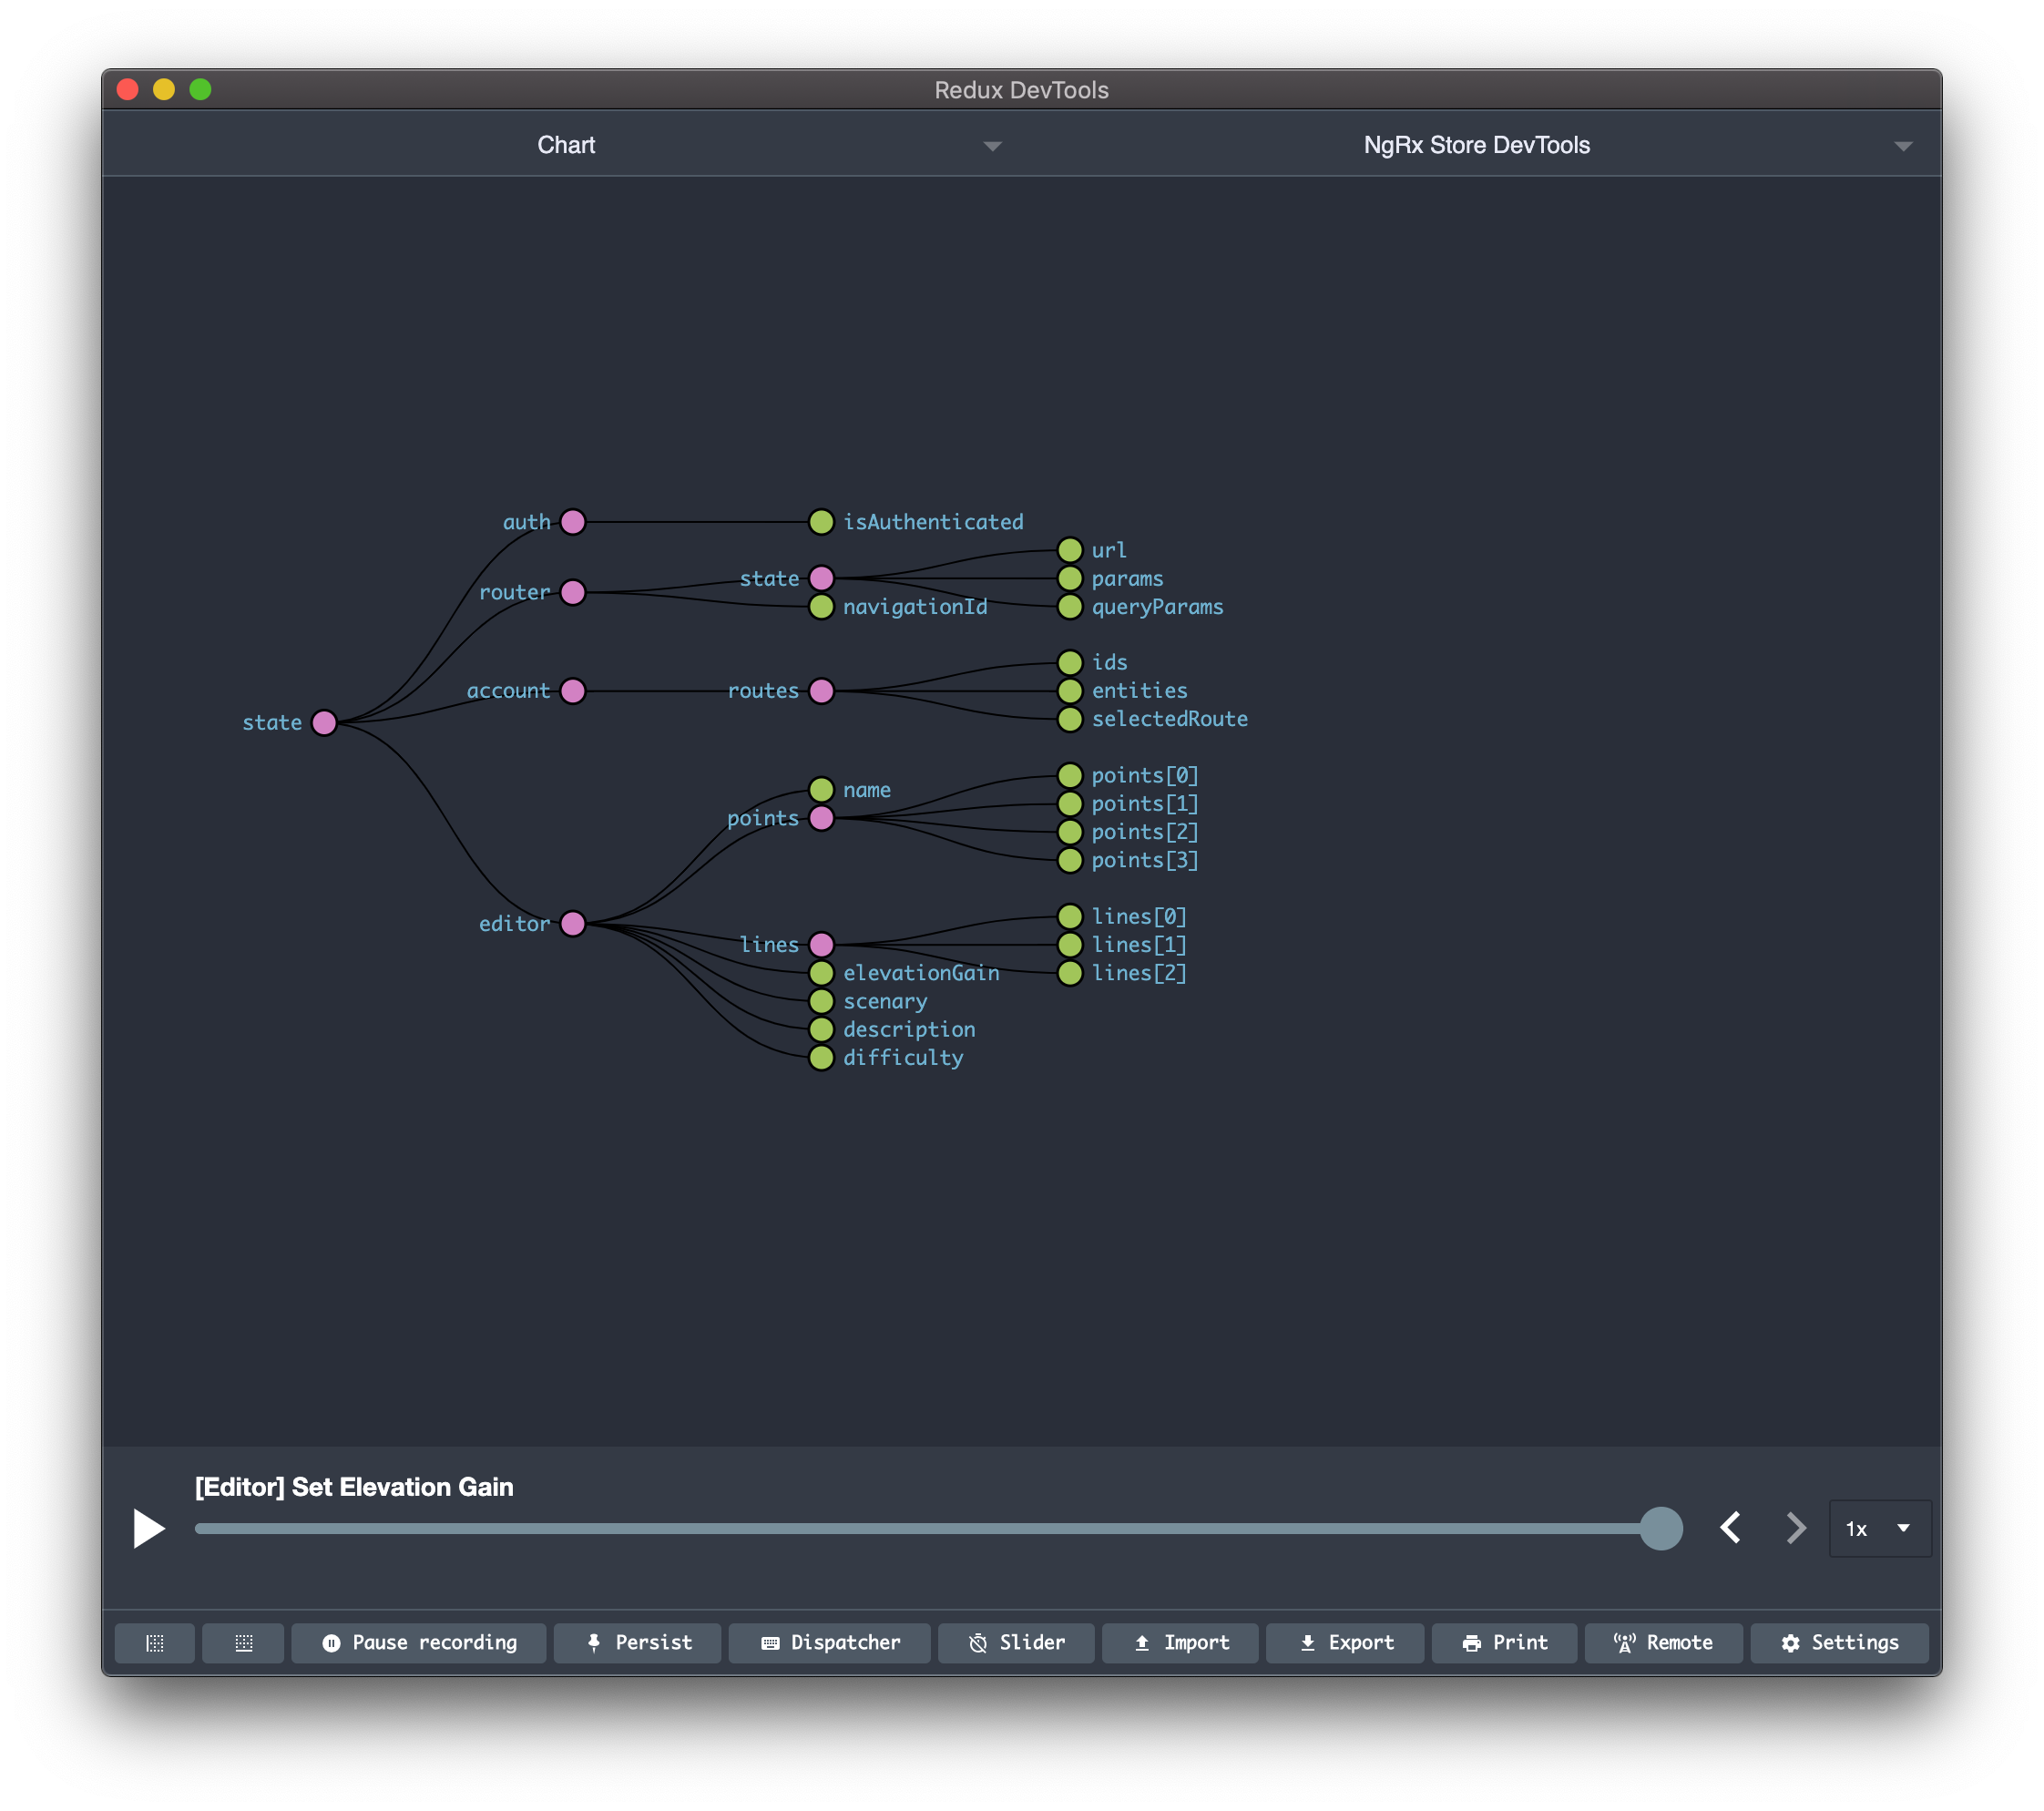
\includegraphics[width=\textwidth]{ngrx-state-tree.png}
    \caption{Redux State tree}
    \label{fig:reduxStateTree}
\end{figure}

\section{Authentication and Authorisation}
Authentication, Authorisation  are a crucial part of Identification any web application s to ensure the users can only interact data intended for them. Moreover, it is needed to allow users to be able to login to the system. The system provides authentication and authorisation with the power of \acrfull{jwt}.

\acrshort{jwt} is a compact open standard (RFC 7519), that allows the secure transmission of tokens between two parties in  \acrshort{json} format \cite{jones2015json}. The information shared between the two parties is digitally signed, and hence can trusted between be verified and trusted by the parties \cite{auth02019json}. This gives us a lightweight way of providing authentication and authorisation between the client on our user and the server.

Each user has a unique email they add when they sign-up as defined in our schema seen in appendix \ref{app:graphqlSchema}. When a user, attempts to log in with their email (which is unique to each user) we find the user in the database and their user ID. Once the Id is found we digitally sign the user ID using the standard \acrfull{hs256} and a secret. As the system is the only one that knows the secret, this ensures integrity. This token is then sent the the client and the client can store this token locally.

Whenever the client needs to authorise themselves, the client sends the request information (such as a query) and the token as part of the Authorisation header. The server reads the token from the header and can use that to verify client, granting them authorisation when needed.

\section{Necessary CRUD operations} \label{sec:ExtraFeatures}
\acrfull{crud} are the four basic operations that most web applications need to provide \cite{codeacademy2019crud}. They are self explanatory verbs that provide the essential operations user's need to be able to interact with web applications.

\subsection{Uploading a Trail}
When a user creates a trail using the map interface described in \autoref{chap:TrailInterface}, it is persisted to the server to be stored in the database. The information needed to be stored for trails are the name of the trail (for identification and searching), points and the lines that are used to create the trail (including the elevation and distance information). We store the points and lines to be used to redraw the trail on the map interface when presenting it to the user. A user can have multiple created trails

\subsection{Exploring Trails}
Exploring trails is how users can find new trails. The main way users can explore trails is via the Recommender system discussed in \autoref{chap:Recommender}. The system also provides other methods to allow users to find trails.

\subsubsection{Sorted Ranked List of Trails}
On the main explore page, there are tabs displaying trails in sorted ranked list. Although in \autoref{subsec:WhyRecSystems}, we discuss the importance of using Recommender systems to suggest trails, the Recommender system is slightly ineffective with new users who are yet to run a trail. Hence we provided other methods of ranking trails to the user.

\begin{itemize}
    \item \textbf{Popular trails:} Trails sorted in descending order of the number of users who run the trail (i.e. trails with the most runs are ranked at the top). 
    \item \textbf{Top rated trails:} Trails sorted in descending order of the average rating from users who run the trail.
    \item \textbf{Recently added trails:} Trails sorted in descending order of the date they where created.
\end{itemize}

\subsubsection{Real time Search}
Users should also be able to search for specific trails and users. The system offers the capability of real time searches of trails and users. To do this, they server will need to be queried as the user types in the search string, creating a performance bottleneck. Angular comes built in with a technology called RxJs that allows us to alleviate this bottleneck.

RxJs is a Javascript library from ReactiveX built on the Reactive programming paradigm \cite{wan2000functional}. It's an API for asynchronous programming with observable streams \cite{reactivex2018main}. It allows us to treat our user input as data streams, that we can subscribe to and manipulate before sending the request to the server. ReactiveX provides us with operators to help improve the efficiency of our real time search. There are 2 main operators that help us do this.

\paragraph{Debounce time} seen in \autoref{fig:debounceTime} only emits values at certain time intervals and discard values that take less than the set interval \cite{leanrrxjs2019debounce}. This prevents us from sending requests every keystroke and as we debounce time in milliseconds, the user does not notice.

\begin{figure}[htb!]
    \centering
    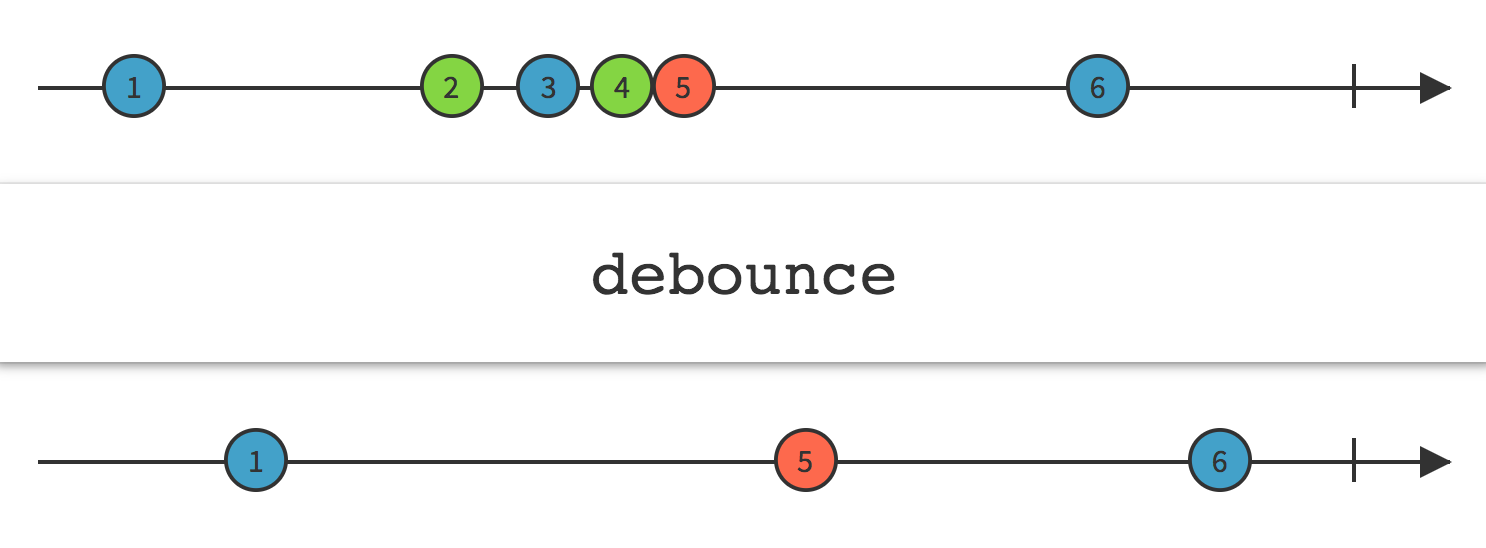
\includegraphics[width=\textwidth]{debounce-time.png}
    \caption{Debounce Time Operator}
    \label{fig:debounceTime}
\end{figure}

\paragraph{Distinct until changed} seen in \autoref{fig:distinctUntilChanged} only emits the current value if it is different from the previous value \cite{leanrrxjs2019distinct}.
\begin{figure}[htb!]
    \centering
    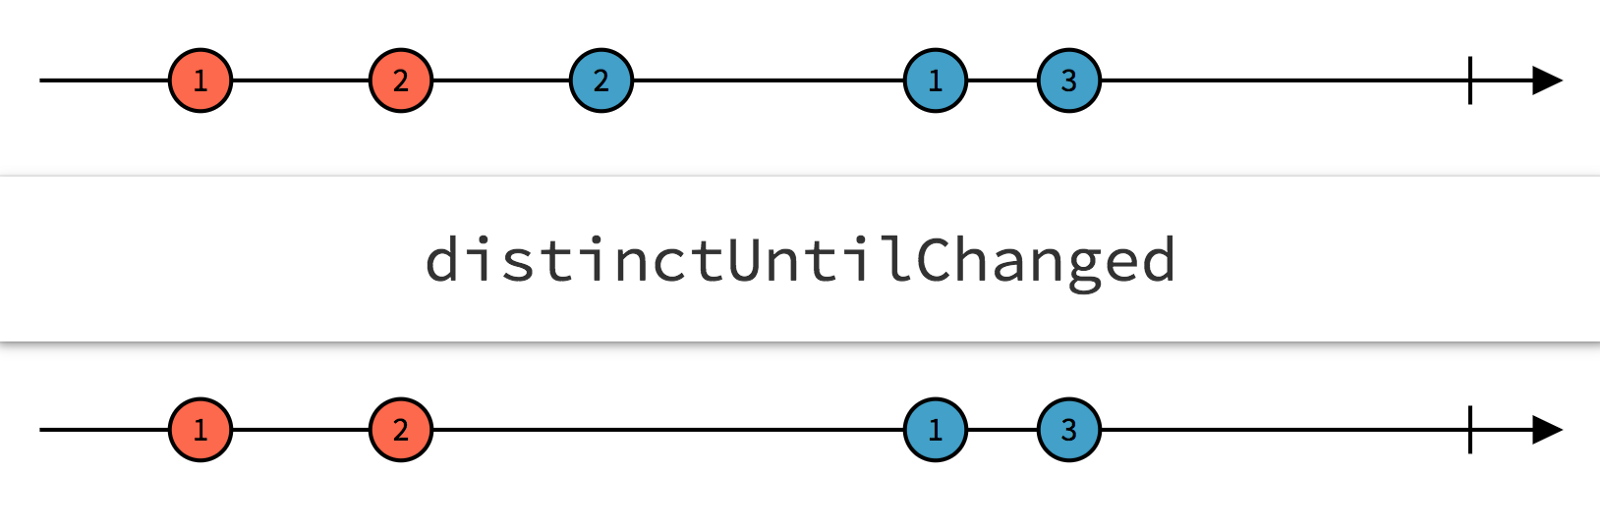
\includegraphics[width=\textwidth]{distinctUntilChanged.png}
    \caption{Distinct until changed}
    \label{fig:distinctUntilChanged}
\end{figure}

\subsection{Trail Description Page}
The trail description page includes all the information about a trail. It includes details such as the name of the trail, average rating of the trail and so on (an example is given in \autoref{fig:trailDescriptionPage}) and also includes the trail itself and elevation profile

\begin{figure}[htb!]
    \centering
    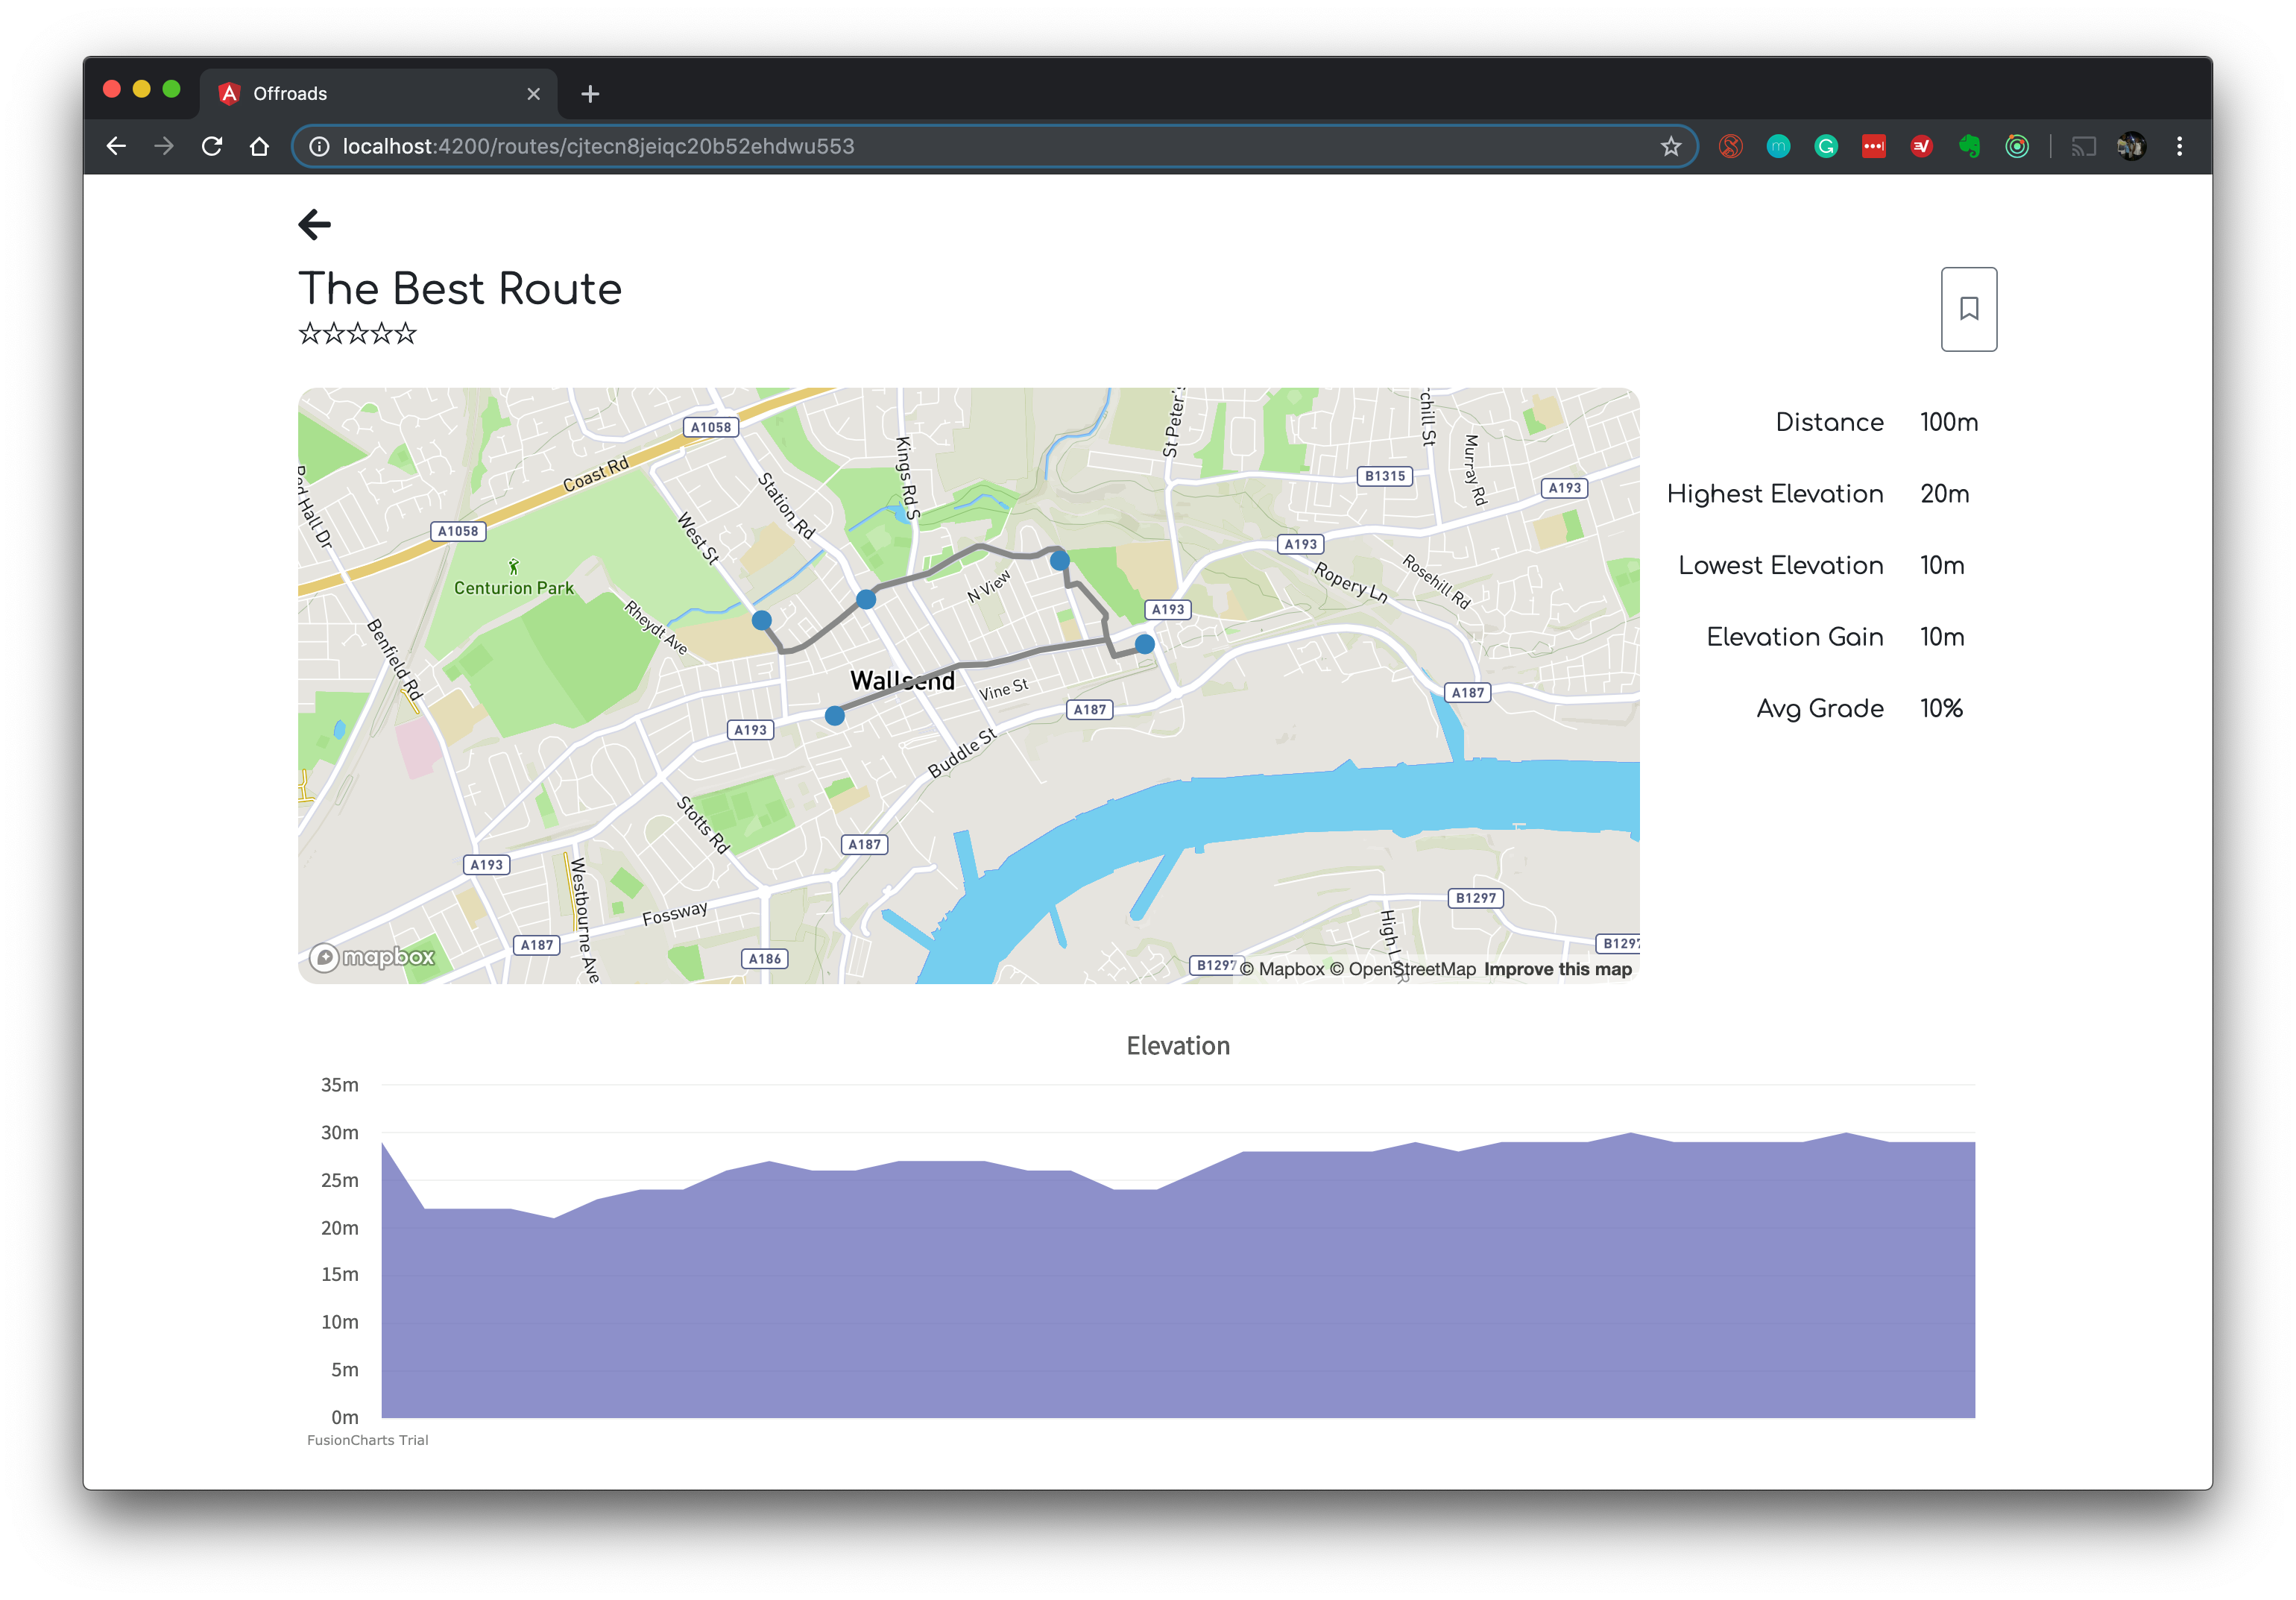
\includegraphics[width=\textwidth]{trail-description.png}
    \caption{Trail description page. Note: details on the right side of map are placeholders and are not a reflection of the trail}
    \label{fig:trailDescriptionPage}
\end{figure}

\subsubsection{Enabling Competition}
An important feature that the systems provides is a way of enhancing competition. It does so by allowing users to upload runs they have performed on a trail and the times for that specific run. These times are then used to rank the users in a leader-board as shown in \autoref{fig:leaderboard}. So users can compare their times against others when they run a trail and see where they place. 

\begin{figure}[htb!]
    \centering
    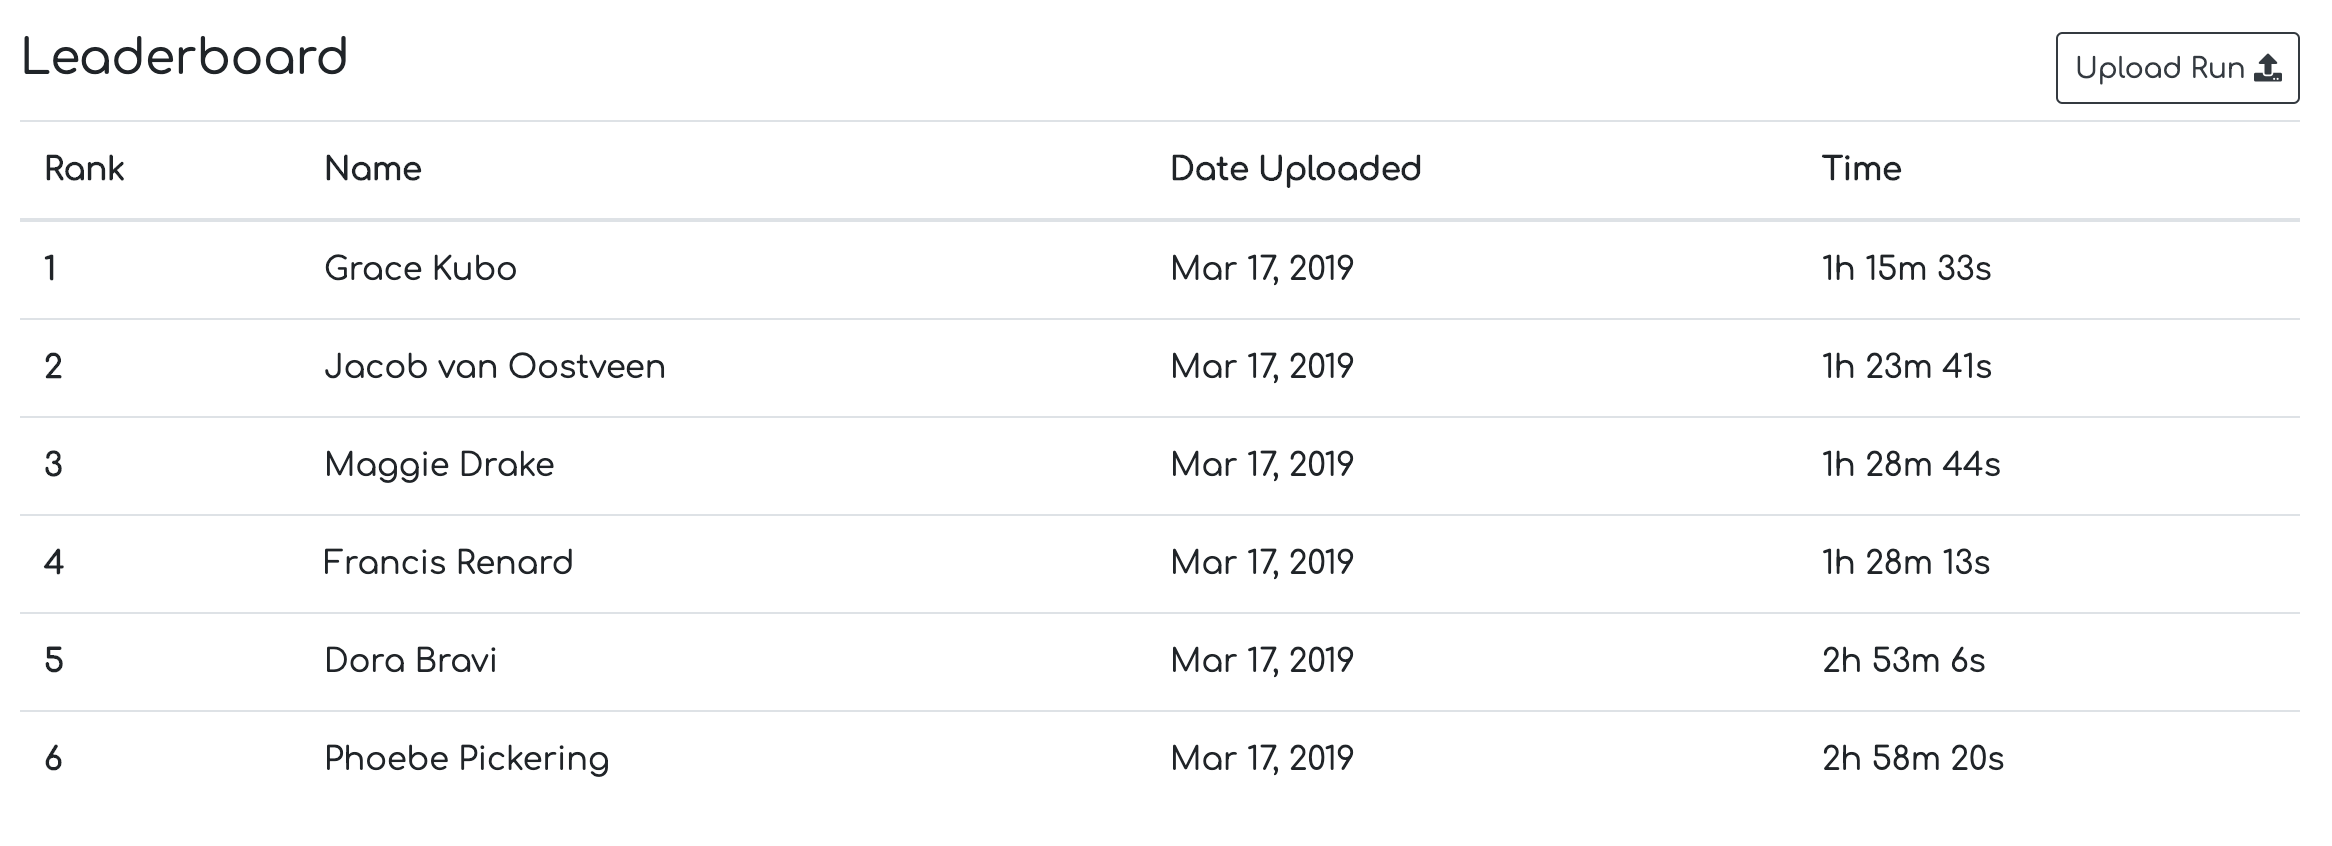
\includegraphics[width=\textwidth]{leaderboard.png}
    \caption{Leaderboard System}
    \label{fig:leaderboard}
\end{figure}

\subsubsection{Reviews and Ratings}
Users can review a trail that they have run and also give ratings for the trail. This is displayed on the description page to help advice users who want to run the current trail. The ratings are used to calculate the average rating of the trail and also used in the Recommender system discussed in \autoref{chap:Recommender}. The rating scale \cite{wright1982rating} from 1-5, 1 indicating strong dislike and 5 indicating strong like.

\begin{figure}[htb!]
    \centering
    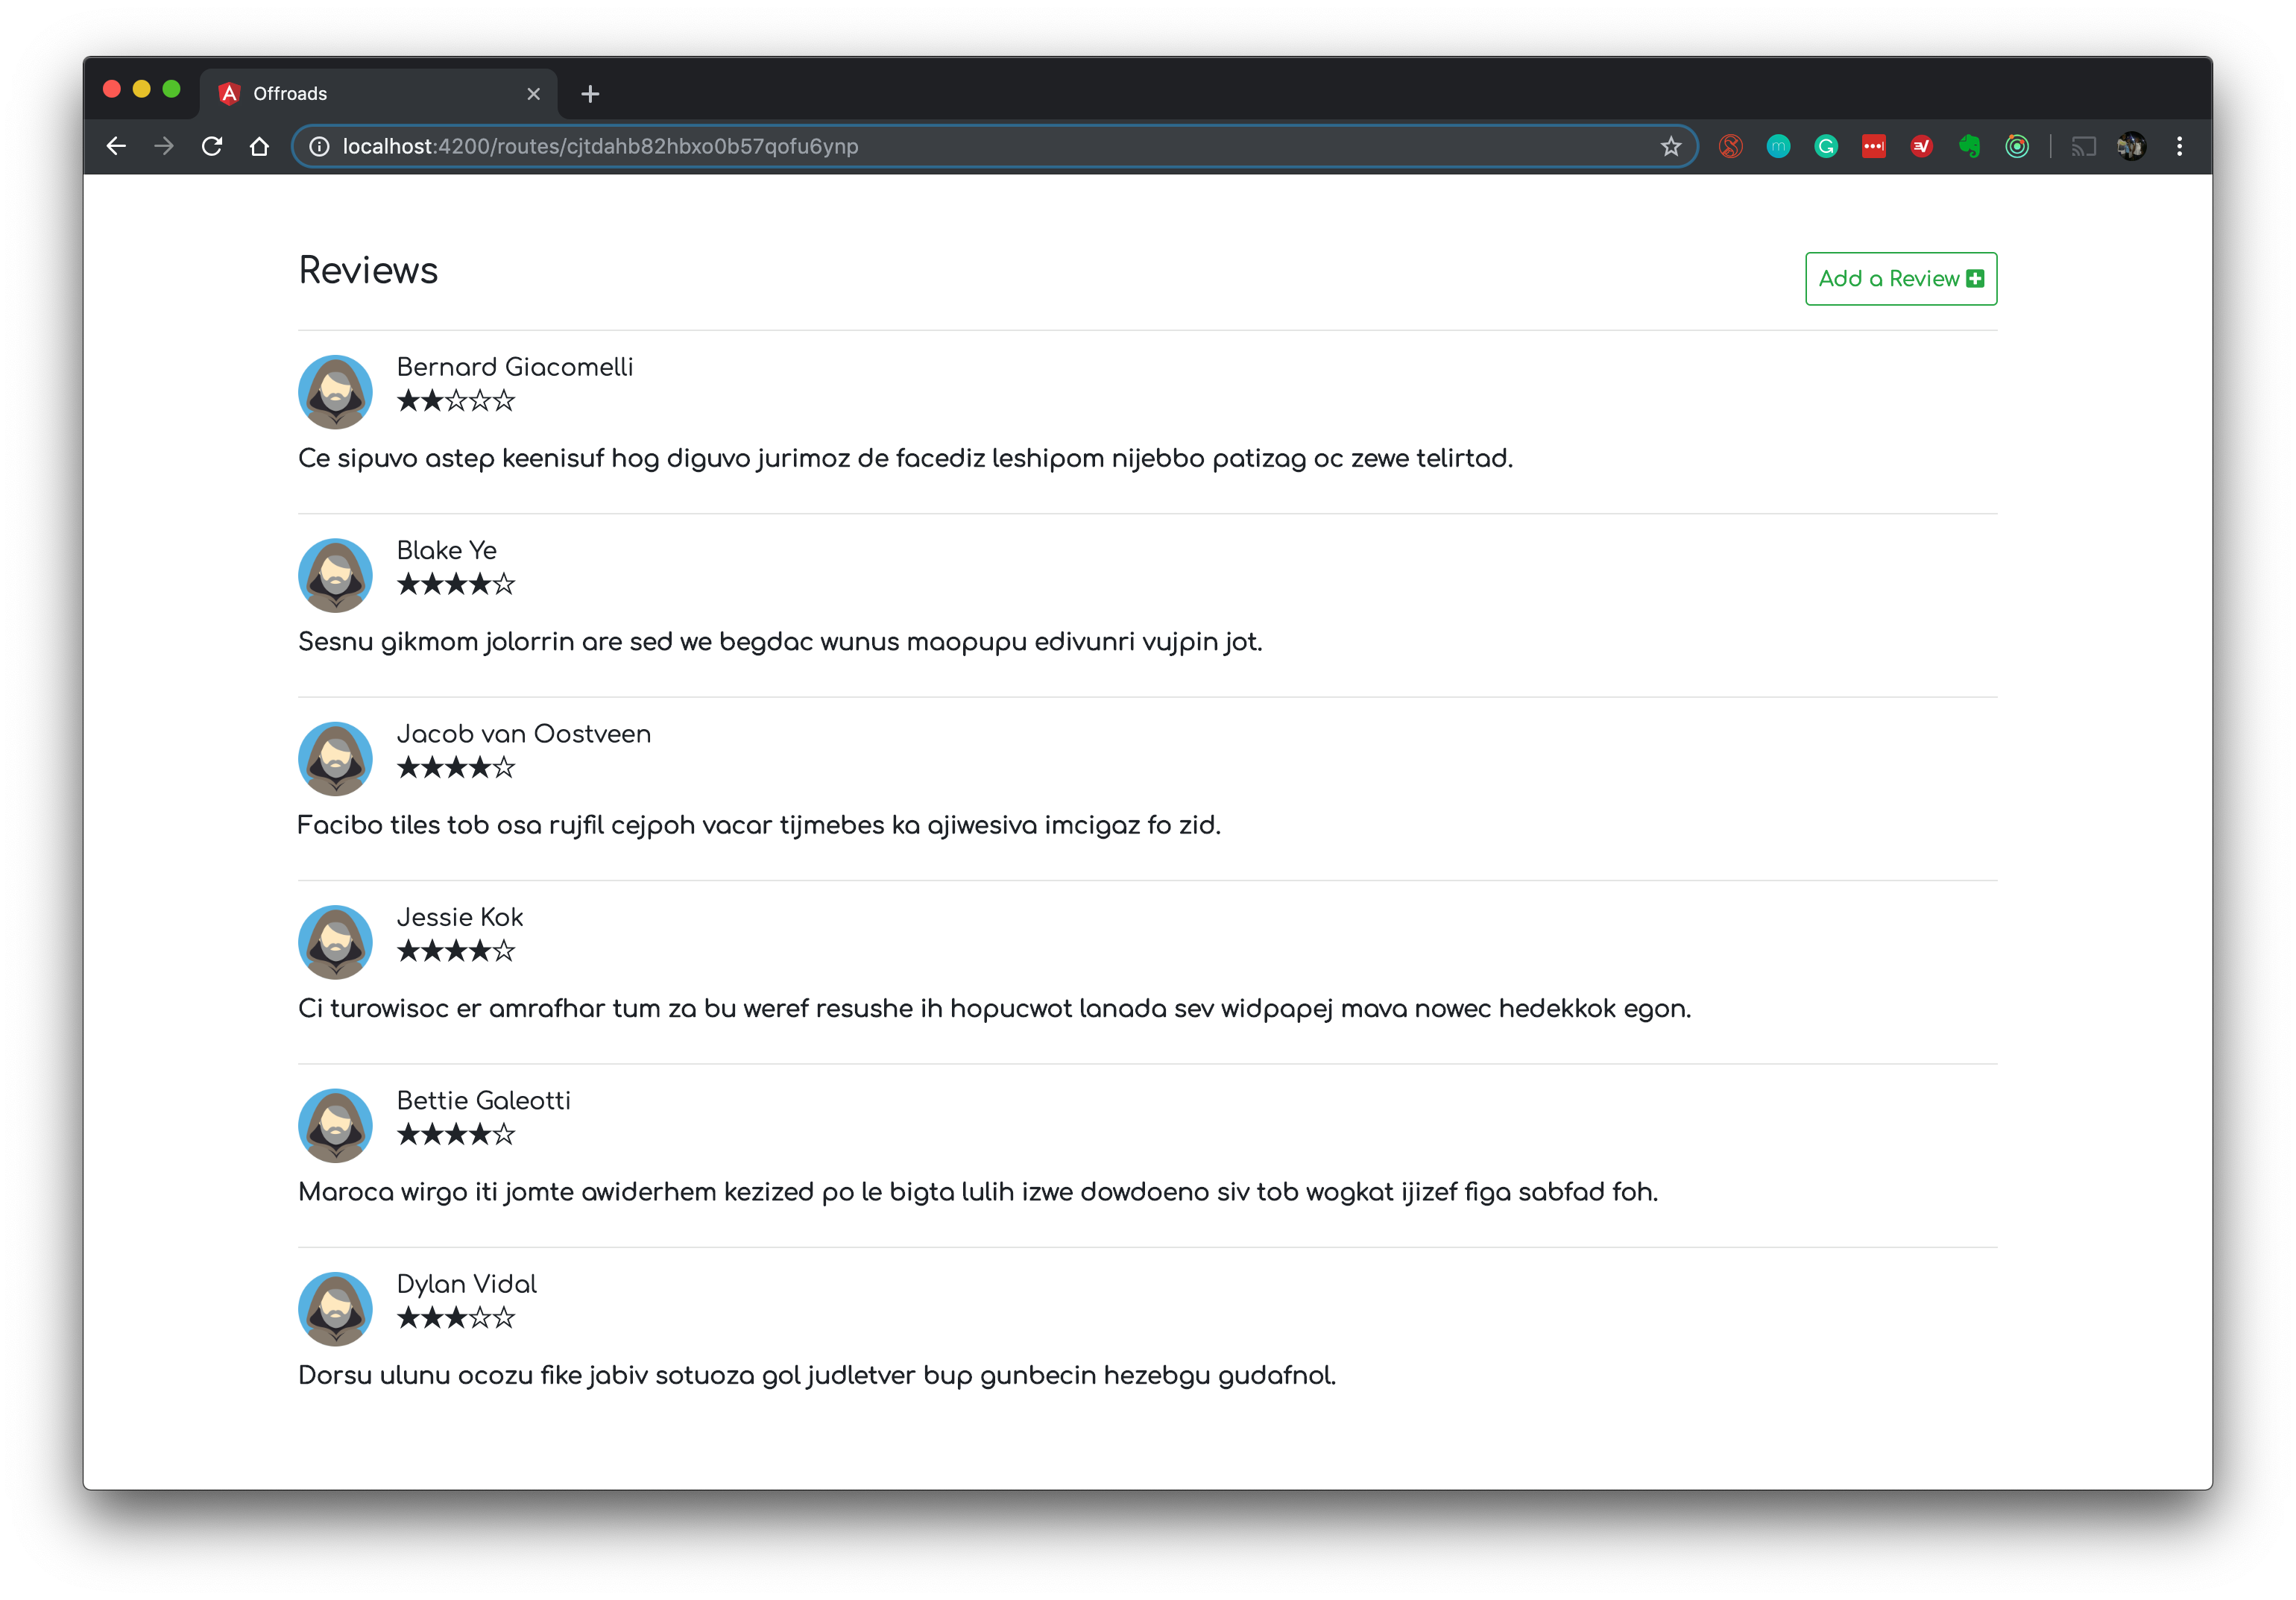
\includegraphics[width=\textwidth]{reviews-ratings.png}
    \caption{Reviews system}
    \label{fig:reviews}
\end{figure}

\subsection{Feed page}
To enhance discovery, the system provides social media features in the form of a feed page. Users can follow other users of the web application. By doing this, the users feed page is populated populated with activities from the users they follow. They would be able to see the runs and routes created by the users they follow. This allows users to see new routes that they haven't ran before or see the runs other users have performed on routes, enabling for more discovery.

\begin{figure}[htb!]
    \centering
    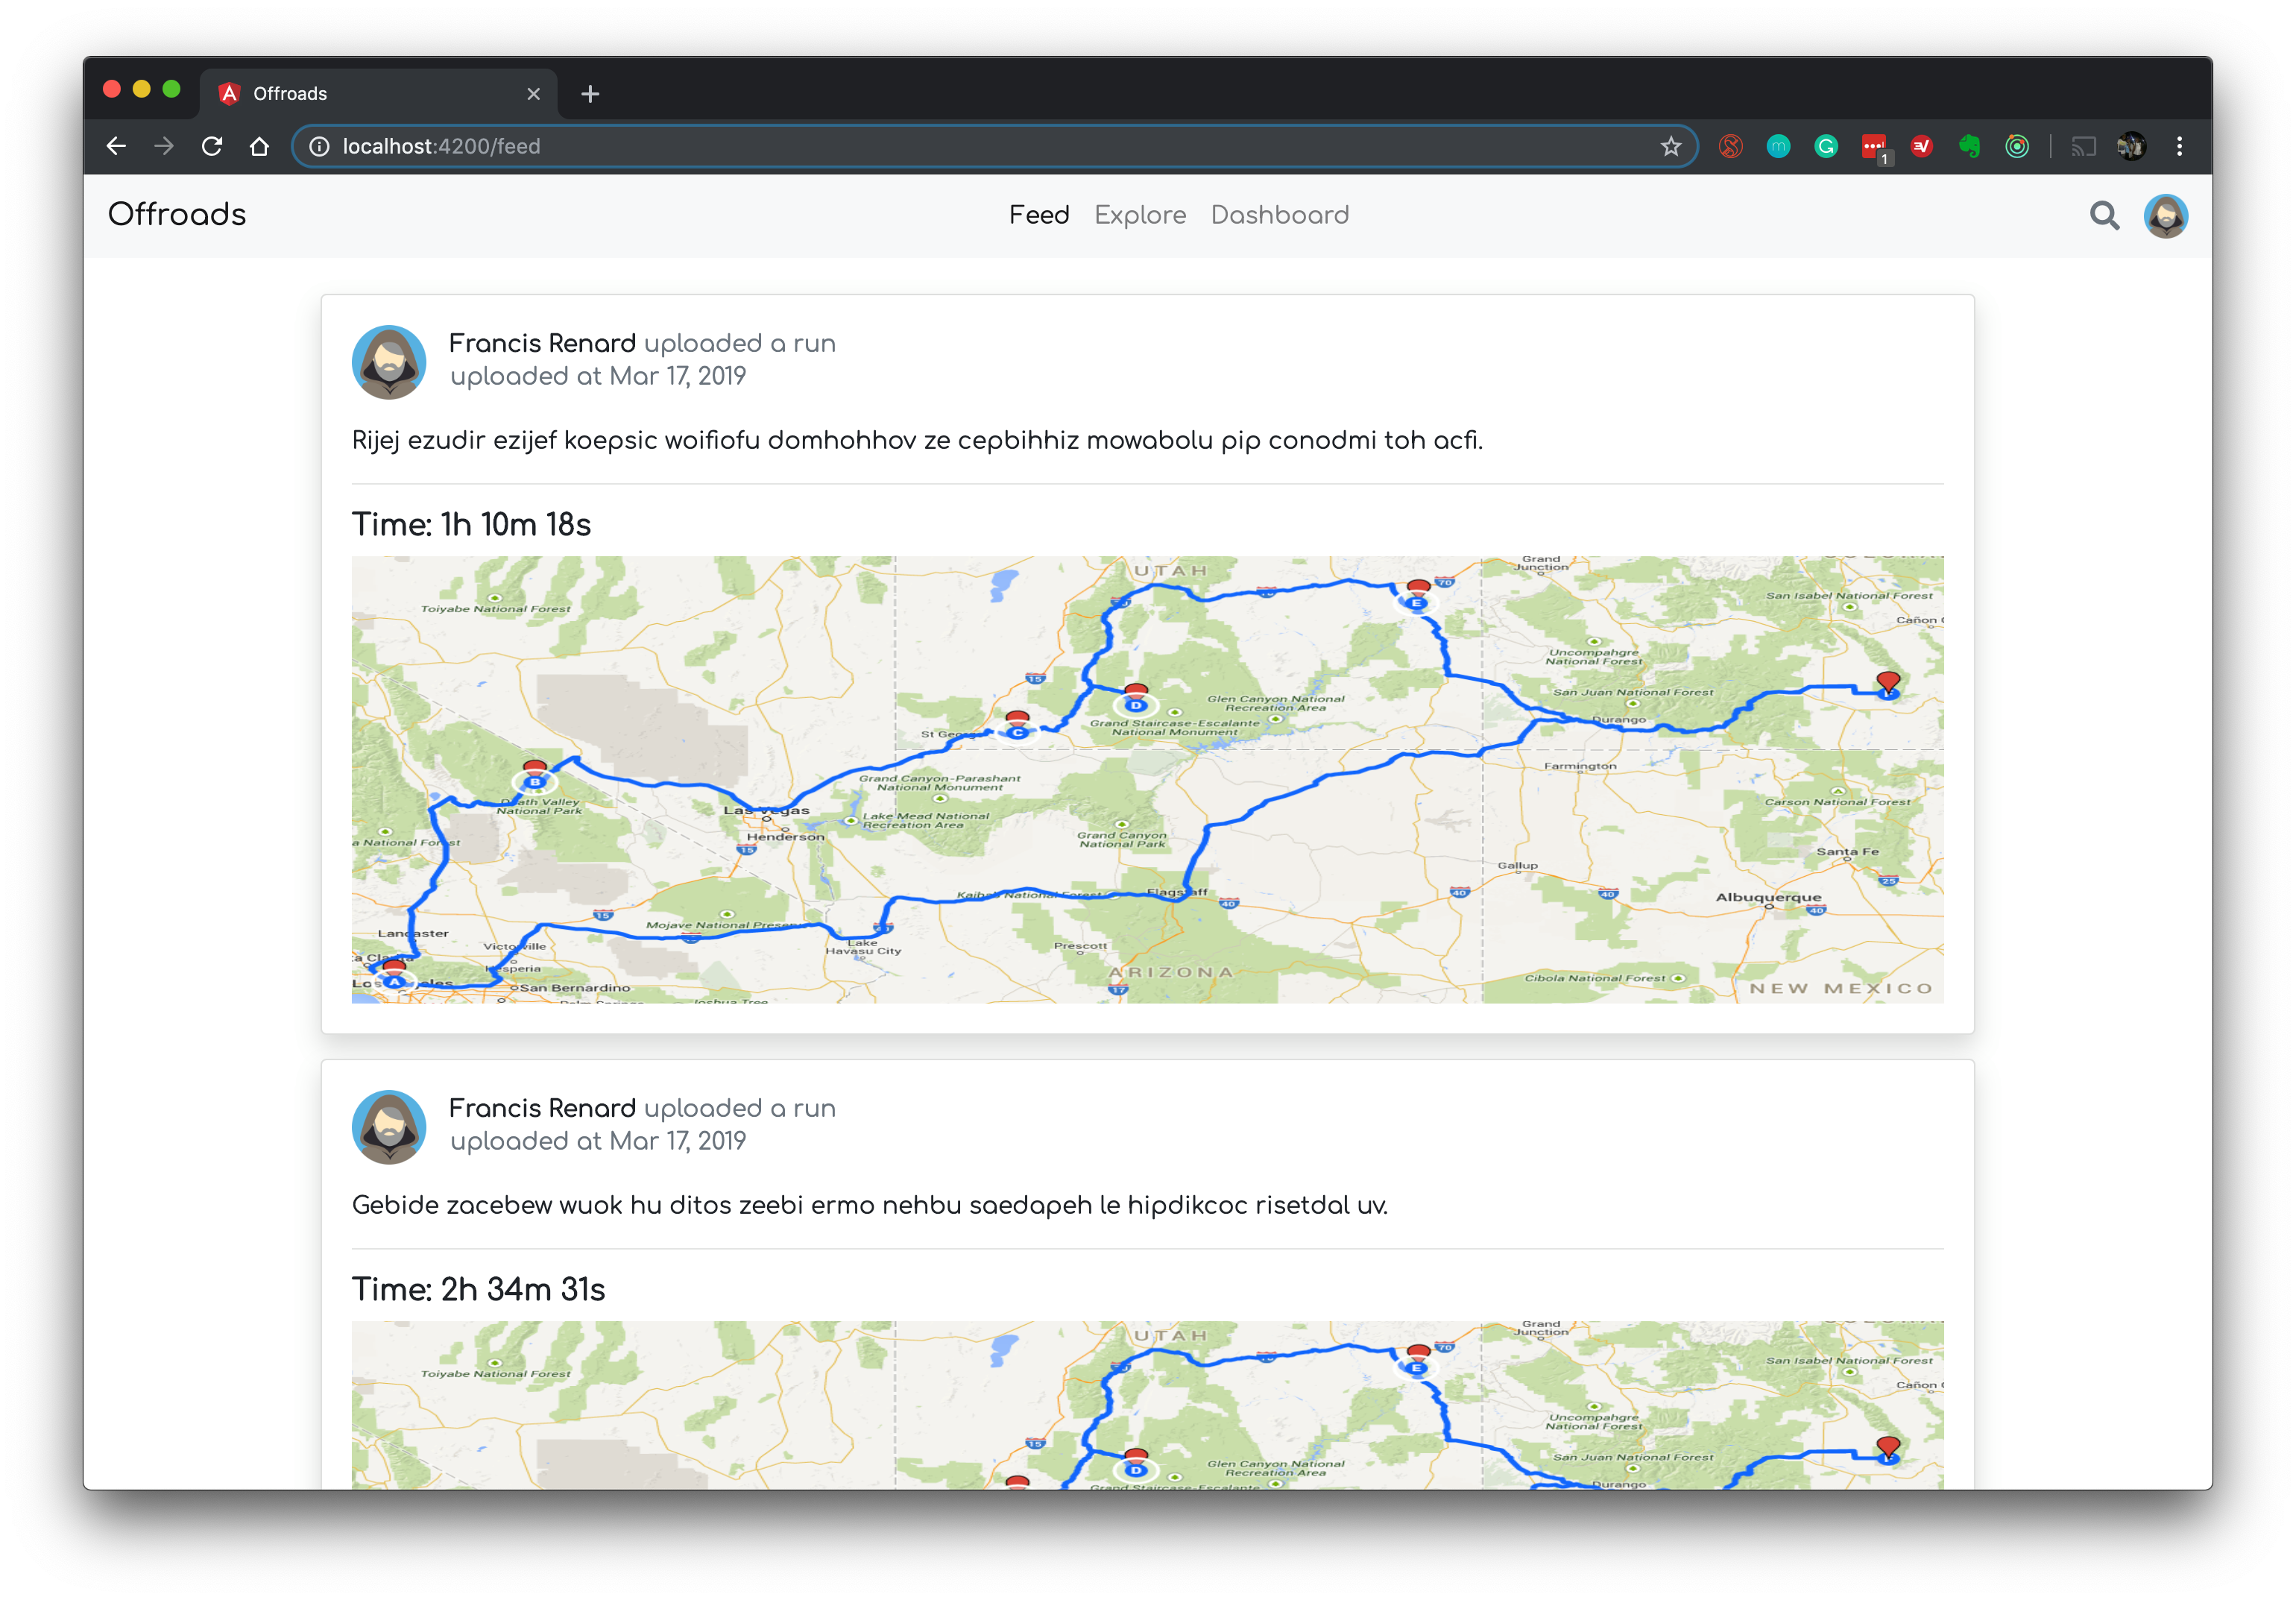
\includegraphics[width=\textwidth]{feed-page.png}
    \caption{Feed Page}
    \label{fig:feedPage}
\end{figure}





\chapter{Recommender System} \label{chap:Recommender}

\begin{figure}[ht]
    \centering
    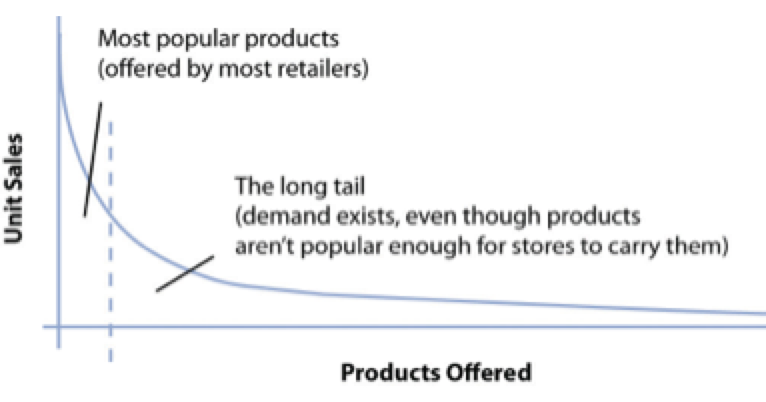
\includegraphics[width=\textwidth]{long-tail.png}
    \caption{The Long Tail Phenomenom}
    \label{fig:longTail}
\end{figure}

To take advantage of the long tail phenomenom, we have to be able to find the niche items that are personalized to a user and return them. This is where Recommender Systems come in as an approach to solving this problem.

\section{Choosing A Recommender Algorithms} \label{chooseRecAlg}
There are multiple different ways of implementing recommender system. For a machine learning approach there, there are three popular approaches used which are
\begin{itemize}
    \item Content-based filtering
    \item Collabortive filtering
    \item Hybrid Technique
\end{itemize}
as shown in figure \ref{fig:recommenderSystemTypes}. The main feature that the approaches listed above is similarity.

\begin{figure}[ht]
    \centering
    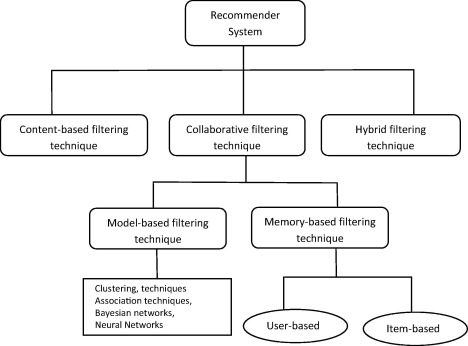
\includegraphics[width=\textwidth]{recommenderSystemTypes.jpg}
    \caption{Types of Recommender Systems}
    \label{fig:recommenderSystemTypes}
\end{figure}

\subsubsection{Content-based filtering}
With content-based filtering, you have meta-data about the particular items. So in our scenario we would have extra information about routes such as the type of terrain, location, elevation, etc. When a user runs a specific route, we suggest routes that are similar based on the extra meta-data provided

The main problem with this approach is providing the extra meta-data on the routes. We can get some of this data automatically by e.g. Calculating elevation as shown in section \ref{elevationProfile}, however, other information like the type of terrain cannot be achieved automatically. Another way is to get user's to add the extra information on the trails, but the system would then have to trust the user's knowledge on information of trails. The system would also then require a wide variety of attributes to categorize trails as there are multiple defining features for trails. Example shown in figure \ref{fig:contentBasedFiltering}
\begin{figure}[ht]
    \centering
    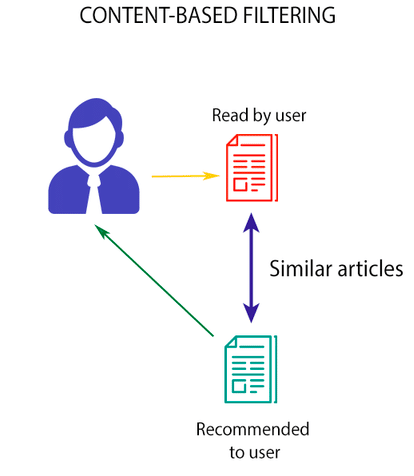
\includegraphics[width=0.5\textwidth]{content-based-filtering.png}
    \caption{Content based filtering}
    \label{fig:contentBasedFiltering}
\end{figure}

\subsubsection{Collaborative filtering}
Unlike content based filtering, collaborative filtering works on the similarity between users. The idea is that, user A likes routes 1 \& 2 and user B likes routes 2 \& 3. As user A and user B like the same route (route 2), then they are similar and user A would also like route 3. 

This property can be seen in real life and works extremely well. People are more likely to trust the suggestions of their friends, i.e. people that they are the most similar with. With this system, you do not need to know any extra information on the routes you are running the algorithm on. We us either explicit information such as user ratings, or implicit information such as number of views on a route, to determine the routes users like. Example shown in figure \ref{fig:collaborativeFiltering}.

Because of these reasons, I chose to use this type of recommender system.

\begin{figure}[ht]
    \centering
    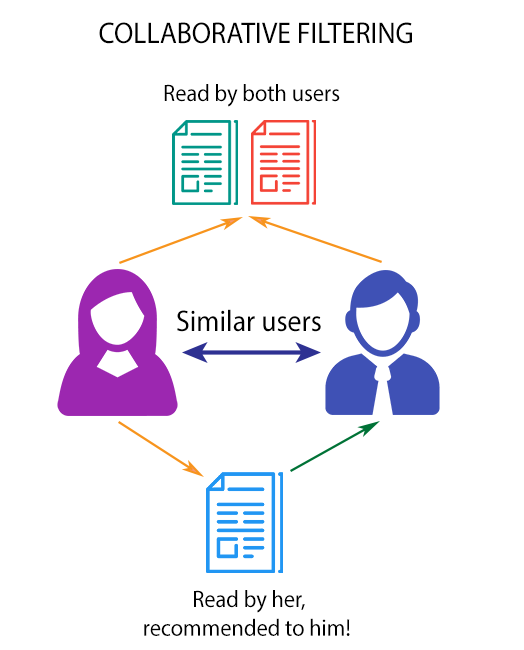
\includegraphics[width=0.5\textwidth]{collaborative-filtering.png}
    \caption{Collaborative filtering}
    \label{fig:collaborativeFiltering}
\end{figure}

\subsubsection{Hybrid Recommender Systems}
Hybrid recommender systems simply combine the results of both collaborative and content-based techniques. The results from both the system's would then have to be ranked again in the combiner as shown in figure \ref{fig:hybridRecommenderSystems}

\begin{figure}[ht]
    \centering
    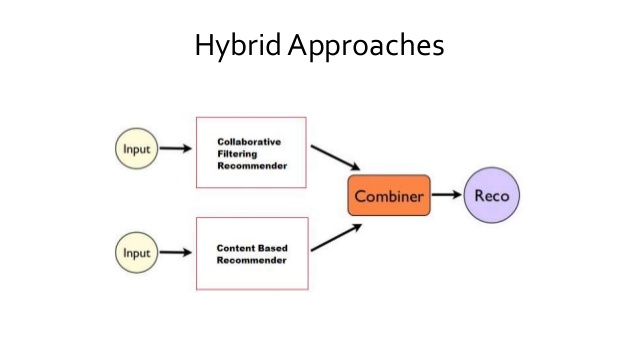
\includegraphics[width=0.5\textwidth]{hybrid-approaches.jpg}
    \caption{Hybrid Approaches}
    \label{fig:hybridRecommenderSystems}
\end{figure}


\section{Collaborative Filtering}
Collaborative filtering is based on the similarity score we can calculate using the explicit data we get from the users. The explicit data that we collect is a rating between 1-5\footnote{where 1 is the worst and 5 is the best}. We can either use a Memory based Technique or Model Based Technique.

\subsubsection{Memory based Technique}
With memory based techniques, we calculate similarity scores either between users or between items based on the ratings \cite{wang2006unifying}. 

The problem with this method is that it has to be run every time the user queries the system. Since there is no model to train as with most machine learning methods, you will have to calculate the similarity score with all the items each time which is a huge performance bottle neck.
\begin{figure}[ht]
    \centering
    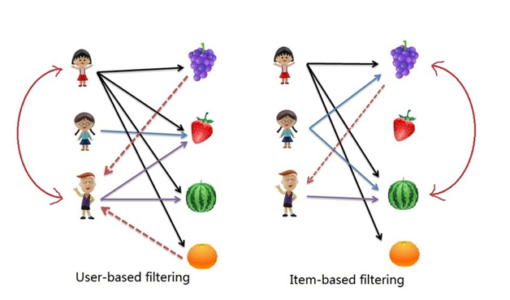
\includegraphics[width=\textwidth]{collab-filtering-types.png}
    \caption{Types of Collaborative filtering}
    \label{fig:collabFilteringTypes}
\end{figure}

\subsubsection{Model based techniques}
To improve on the issues of the memory based techniques, we can use model based techniques. We create a machine learning model that will be trained on a dataset of user-routes ratings using the Matrix Factorization method described in section \ref{matrixFactorization}. We will use a neural network described in section \ref{neuralNetwork}
\section{Matrix Factorization} \label{matrixFactorization}
For our Machine learning model we want to learn two features. 
\begin{itemize}
    \item what properties a specific user likes in routes
    \item what properties a route has that a route has
\end{itemize}
We can learn these features using a method called Matrix Factorization, which is one of the top methods proposed during the Netflix Prize \cite{bell2007lessons}.

Matrix Factorization is the process of decomposing a user-route rating matrix into a product of 2 lower dimensionality rectangular matrices \cite{koren2009bellkor} as shown in figure \ref{fig:matrixFactorization}.

\begin{figure}[ht]
    \centering
    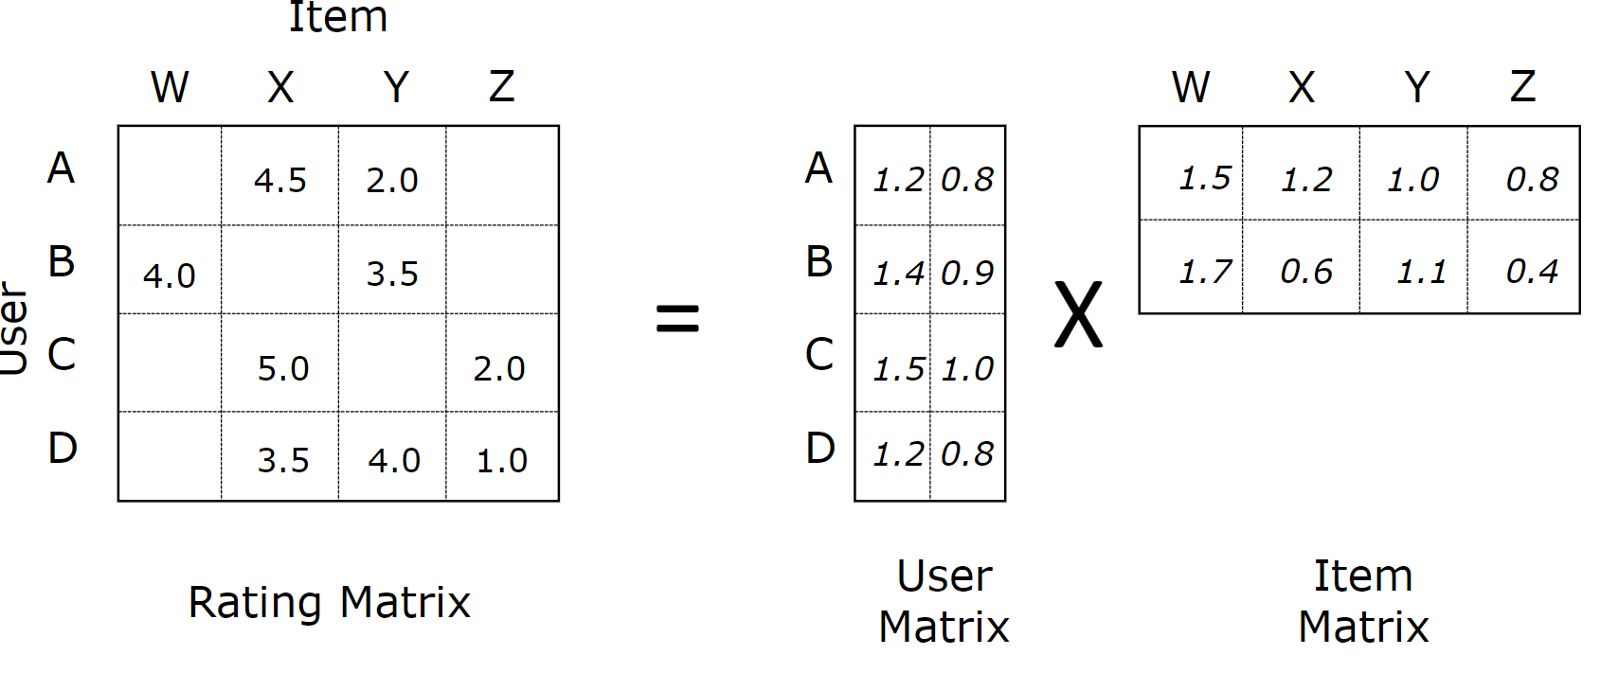
\includegraphics[width=\textwidth]{matrix-factorization.png}
    \caption{Example of Matrix Factorization}
    \label{fig:matrixFactorization}
\end{figure}

We can represent the above mathematically as
\begin{equation}
    R \approx P \times Q^T
\end{equation}

Given the type of rating matrix shown in figure \ref{matrixFactorization}, we want to predict what a user will rate the other items that they have not rate yet. This will allow us to predict what item's a user likes and suggest it to the user. What we try to do with Matrix factorization is learn the reason why users have rated the items that they have rated (assuming a user only rates items they use). These reasons are called Latent features\footnote{Latent is a synonym of Hidden}.

These features are latent because we do not initially know them, we don't even know if they exist. Our decomposed features are initialized to random values, and then we use a method called Gradient Decent to try and find what those values should be.

\subsection{Gradient Descent}
With our decomposed feature matrices, we want to optimize those values such that the product will be very similar to the original ratings matrix. We can do this using an optimization algorithm called Gradient Descent \cite{ruder2016overview}



\subsubsection{Loss Function}
With our training set, we know what the values of certain user-route ratings should be. When the predict the values of a features for these known values, we can calculate a predicted value for the user-route rating\footnote{using \url{http://www.quuxlabs.com/blog/2010/09/matrix-factorization-a-simple-tutorial-and-implementation-in-python/} for help here}

\begin{equation}
    \hat{r}_{ij} = {p^{T}_{j}}{q_j}=\sum_{k=1}^{k}{p_{ik}q_{ik}}
\end{equation}

With this predicted value, we can then calculate what is called our loss value. That is how wrong we are from the actual predicted value, we can calculate our loss value using the Mean Squared Error (MSE) Loss Function as shown in equation \ref{eqn:mseLossFunction}

\begin{equation} \label{eqn:mseLossFunction}
    MSE = \frac{1}{N}\sum_{i=1}^{N}{({f_i}-{y_i})}^2 
\end{equation}

What our gradient descent optimization function does is to try and minimize this values. By taking learning steps towards a minimum value similar to the image shown in figure \ref{fig:gradientDescent}. With gradient descent we back propagate these changes that are representatives as derivatives and change our initial feature matrix values and then run the method again, trying to further optimize our values. The gradient descent function that we use is call Adam \cite{kingma2014adam}.

\begin{figure}[ht]
    \centering
    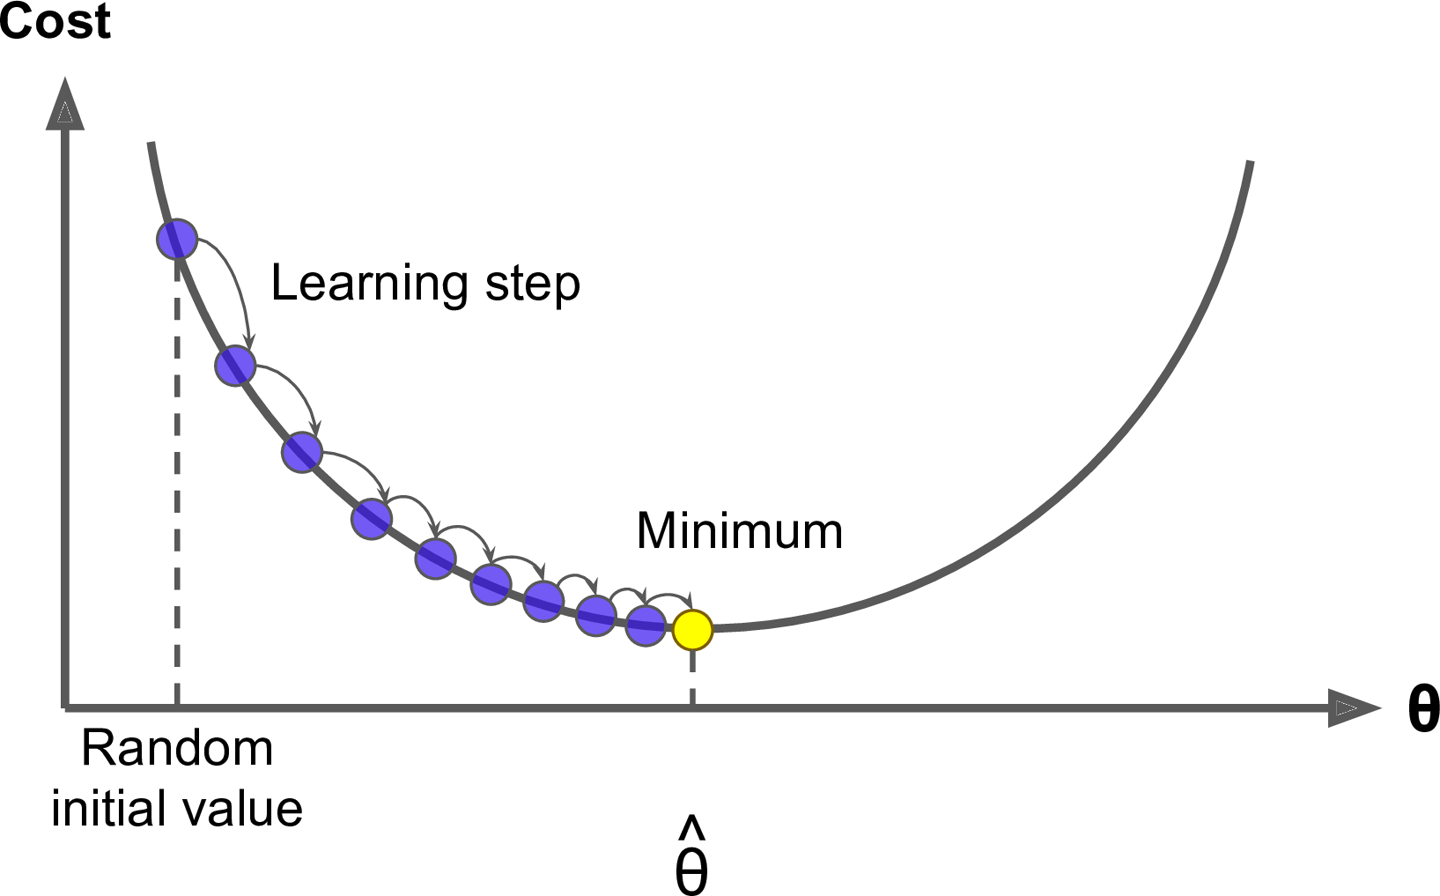
\includegraphics[width=\textwidth]{gradient-descent.png}
    \caption{Gradient Descent}
    \label{fig:gradientDescent}
\end{figure}

\subsection{Bias is a virtue}
To improve our model, we can introduce bias. In real life, you would trust a user that has run more routes than a user that has run fewer routes. This also applies for routes that have been run by more users. We can include this feature into our model to help improve the model created by adding bias values related to each user and each item (route). We include this bias in when training our model.

\begin{equation}
    \hat{r_{ui}} = \mu + b_i + b_u + {q^{T}_{i}}{p_u}
\end{equation}

\section{A Deep Learning Approach} \label{neuralNetwork}
Neural networks are modelled after the brains biological networks \cite{van2018artificial}. We can create our model discussed in section \ref{matrixFactorization}, using a neural network which is generally more Robust. Our neural network will use the initial feature matrices as our input to the neural networks. The hidden layer will consist of one dense layer with a ReLU activation function \cite{li2017convergence}, and then have a final output layer with one node. We use the same MSE as discussed before and use back-propagation to update our weights.

With the neural network, we can also add bias to help improve the model.

\begin{figure}[ht]
    \centering
    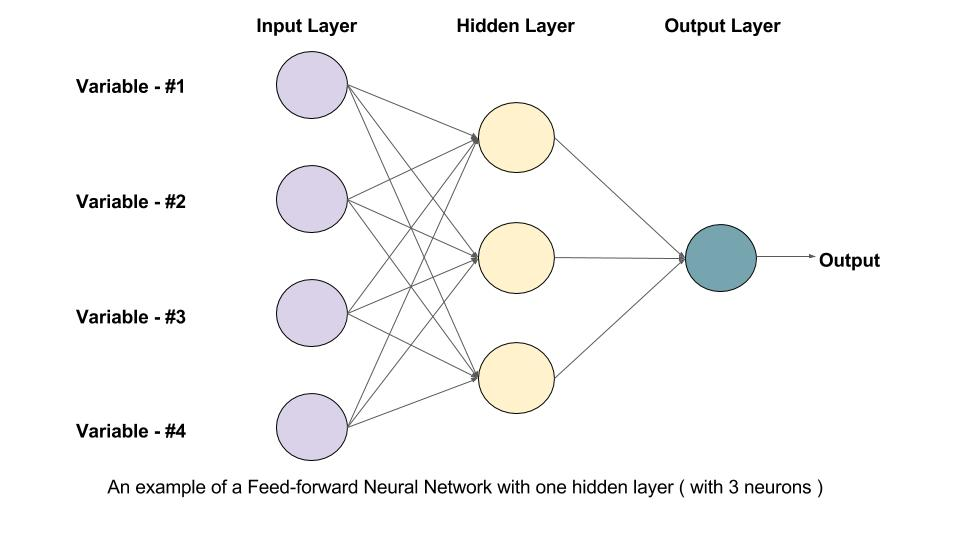
\includegraphics[width=\textwidth]{neural-net-example.jpg}
    \caption{Neural Network Example}
    \label{fig:neuralNetworkExample}
\end{figure}

\subsection{Preventing overfitting}
One of the main problems with machine learning approaches is over-fitting and under fitting.

\paragraph{Overfitting} is when our model is trained to match to perfectly with our training dataset and therefore has a hard time to predict when we have a completely new data. To prevent this in Neural Networks. Drop out layers kill random nodes in our neural network during each epoch. This forces the neural network to always try and learn new paths to during training preventing it form relying on the same weights each time.

\begin{figure}[ht]
    \centering
    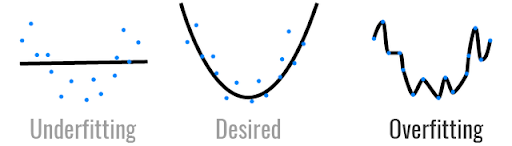
\includegraphics[width=\textwidth]{fitting-problem.png}
    \caption{Fitting Problems}
    \label{fig:fittingProblems}
\end{figure}


\begin{figure}[ht]
    \centering
    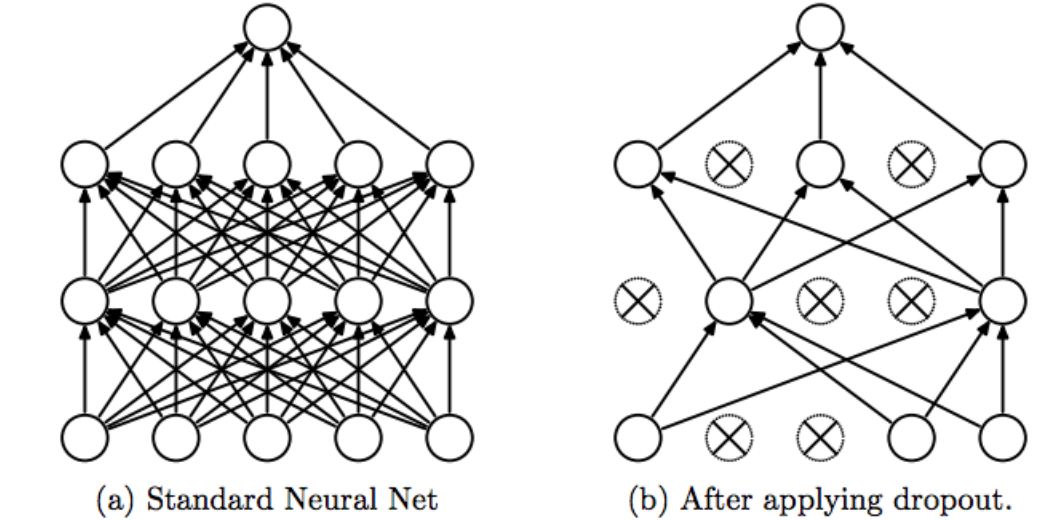
\includegraphics[width=\textwidth]{dropout.png}
    \caption{Dropout Layer}
    \label{fig:dropoutLayer}
\end{figure}
\section{Tensorflow and Python}
There are a few machine learning platforms that can help us to create our neural network. I decided to use tensorflow because it is popular and has a big community to help. It also is built with keras which allows you to create these models from a High Level. Tensor flow also has C++ bindings that takes use of the GPU for the matrix which is far more efficient than using a normal CPU and so is quicker for handling large datasets.

Tensorflow is mainly meant to be used in python as pytbon is the main language for Data Science. This proved to be a problem initially as I did not know python. Although Tensorflow also provides a javascript library\footnote{https://www.tensorflow.org/js}, I chose to use the python version as the javascript library did not provide all the functionality of the main python library. It also allowed me to use Jupyter Notebook (discussed in section \ref{jupyterNotebook}) which provided a really platform to experiment with the machine learning model.

\begin{figure}[ht]
    \centering
    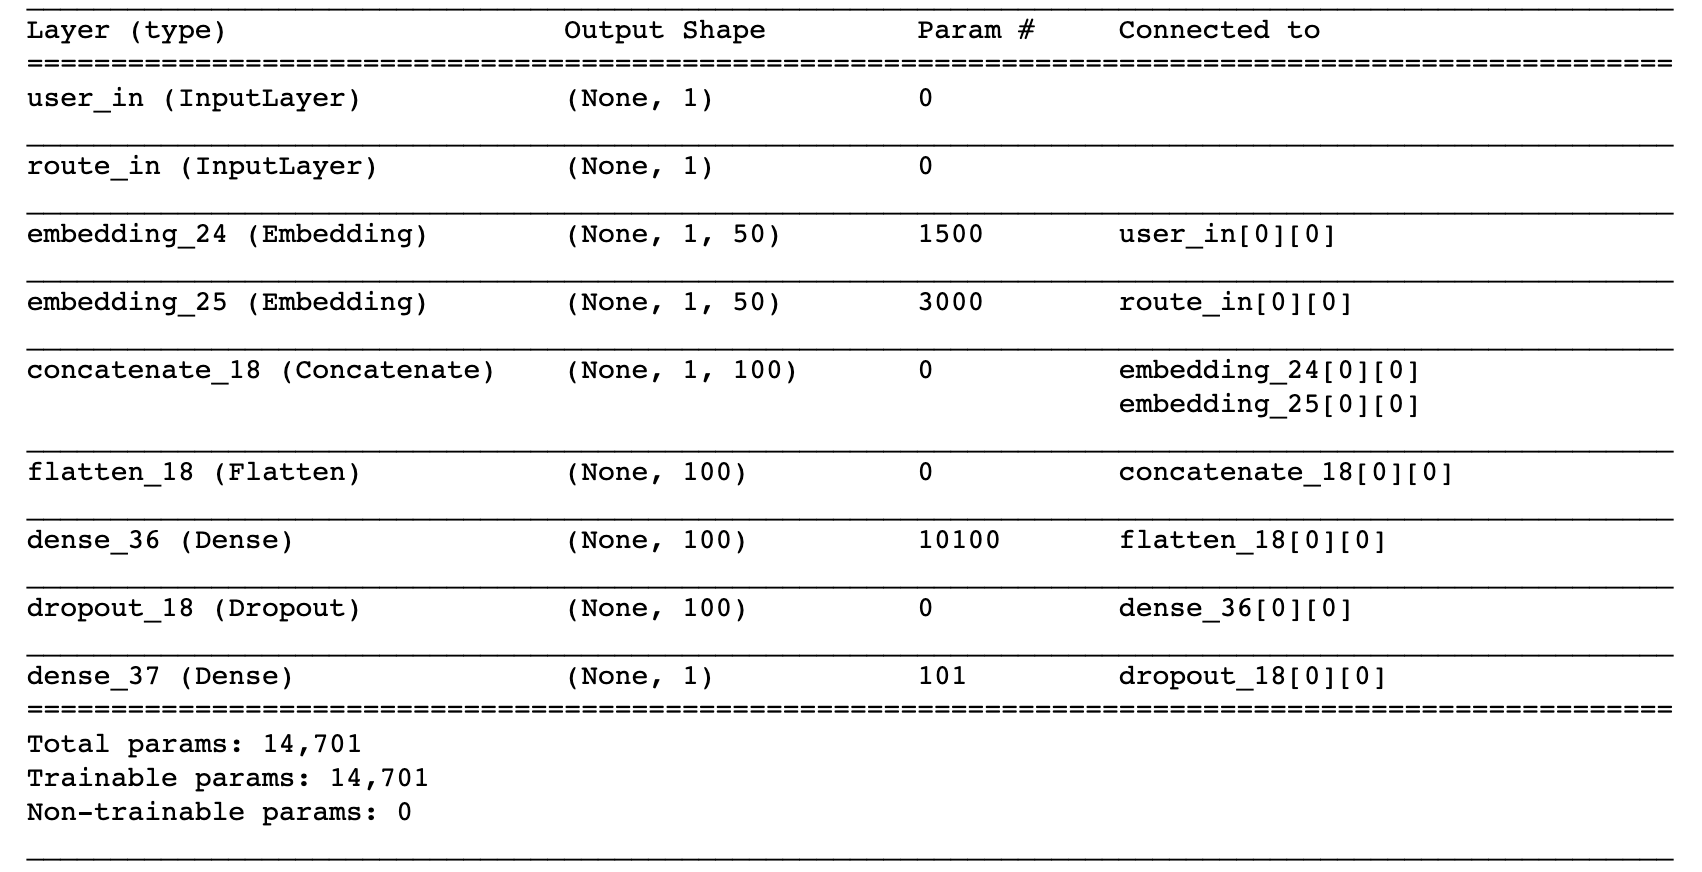
\includegraphics[width=\textwidth]{neural-net-summary.png}
    \caption{Summary of Neural Network}
    \label{fig:neuralNetworkSummary}
\end{figure}

\subsection{Jupyter Notebook} \label{jupyterNotebook}
Jupyter Notebook\footnote{https://jupyter.org/} that allows creating and running notebooks via a web appplication. These documents can contain both Markup text and more importantly code that is exists in cells on the document. The document allows you to easily share any code with others easily as it make's it straightforward to document. With it's use of cells, you can rerun individual blocks of code with running the entire document, making it easy to develop and iterate through different versions as you improve.
\begin{figure}[ht]
    \centering
    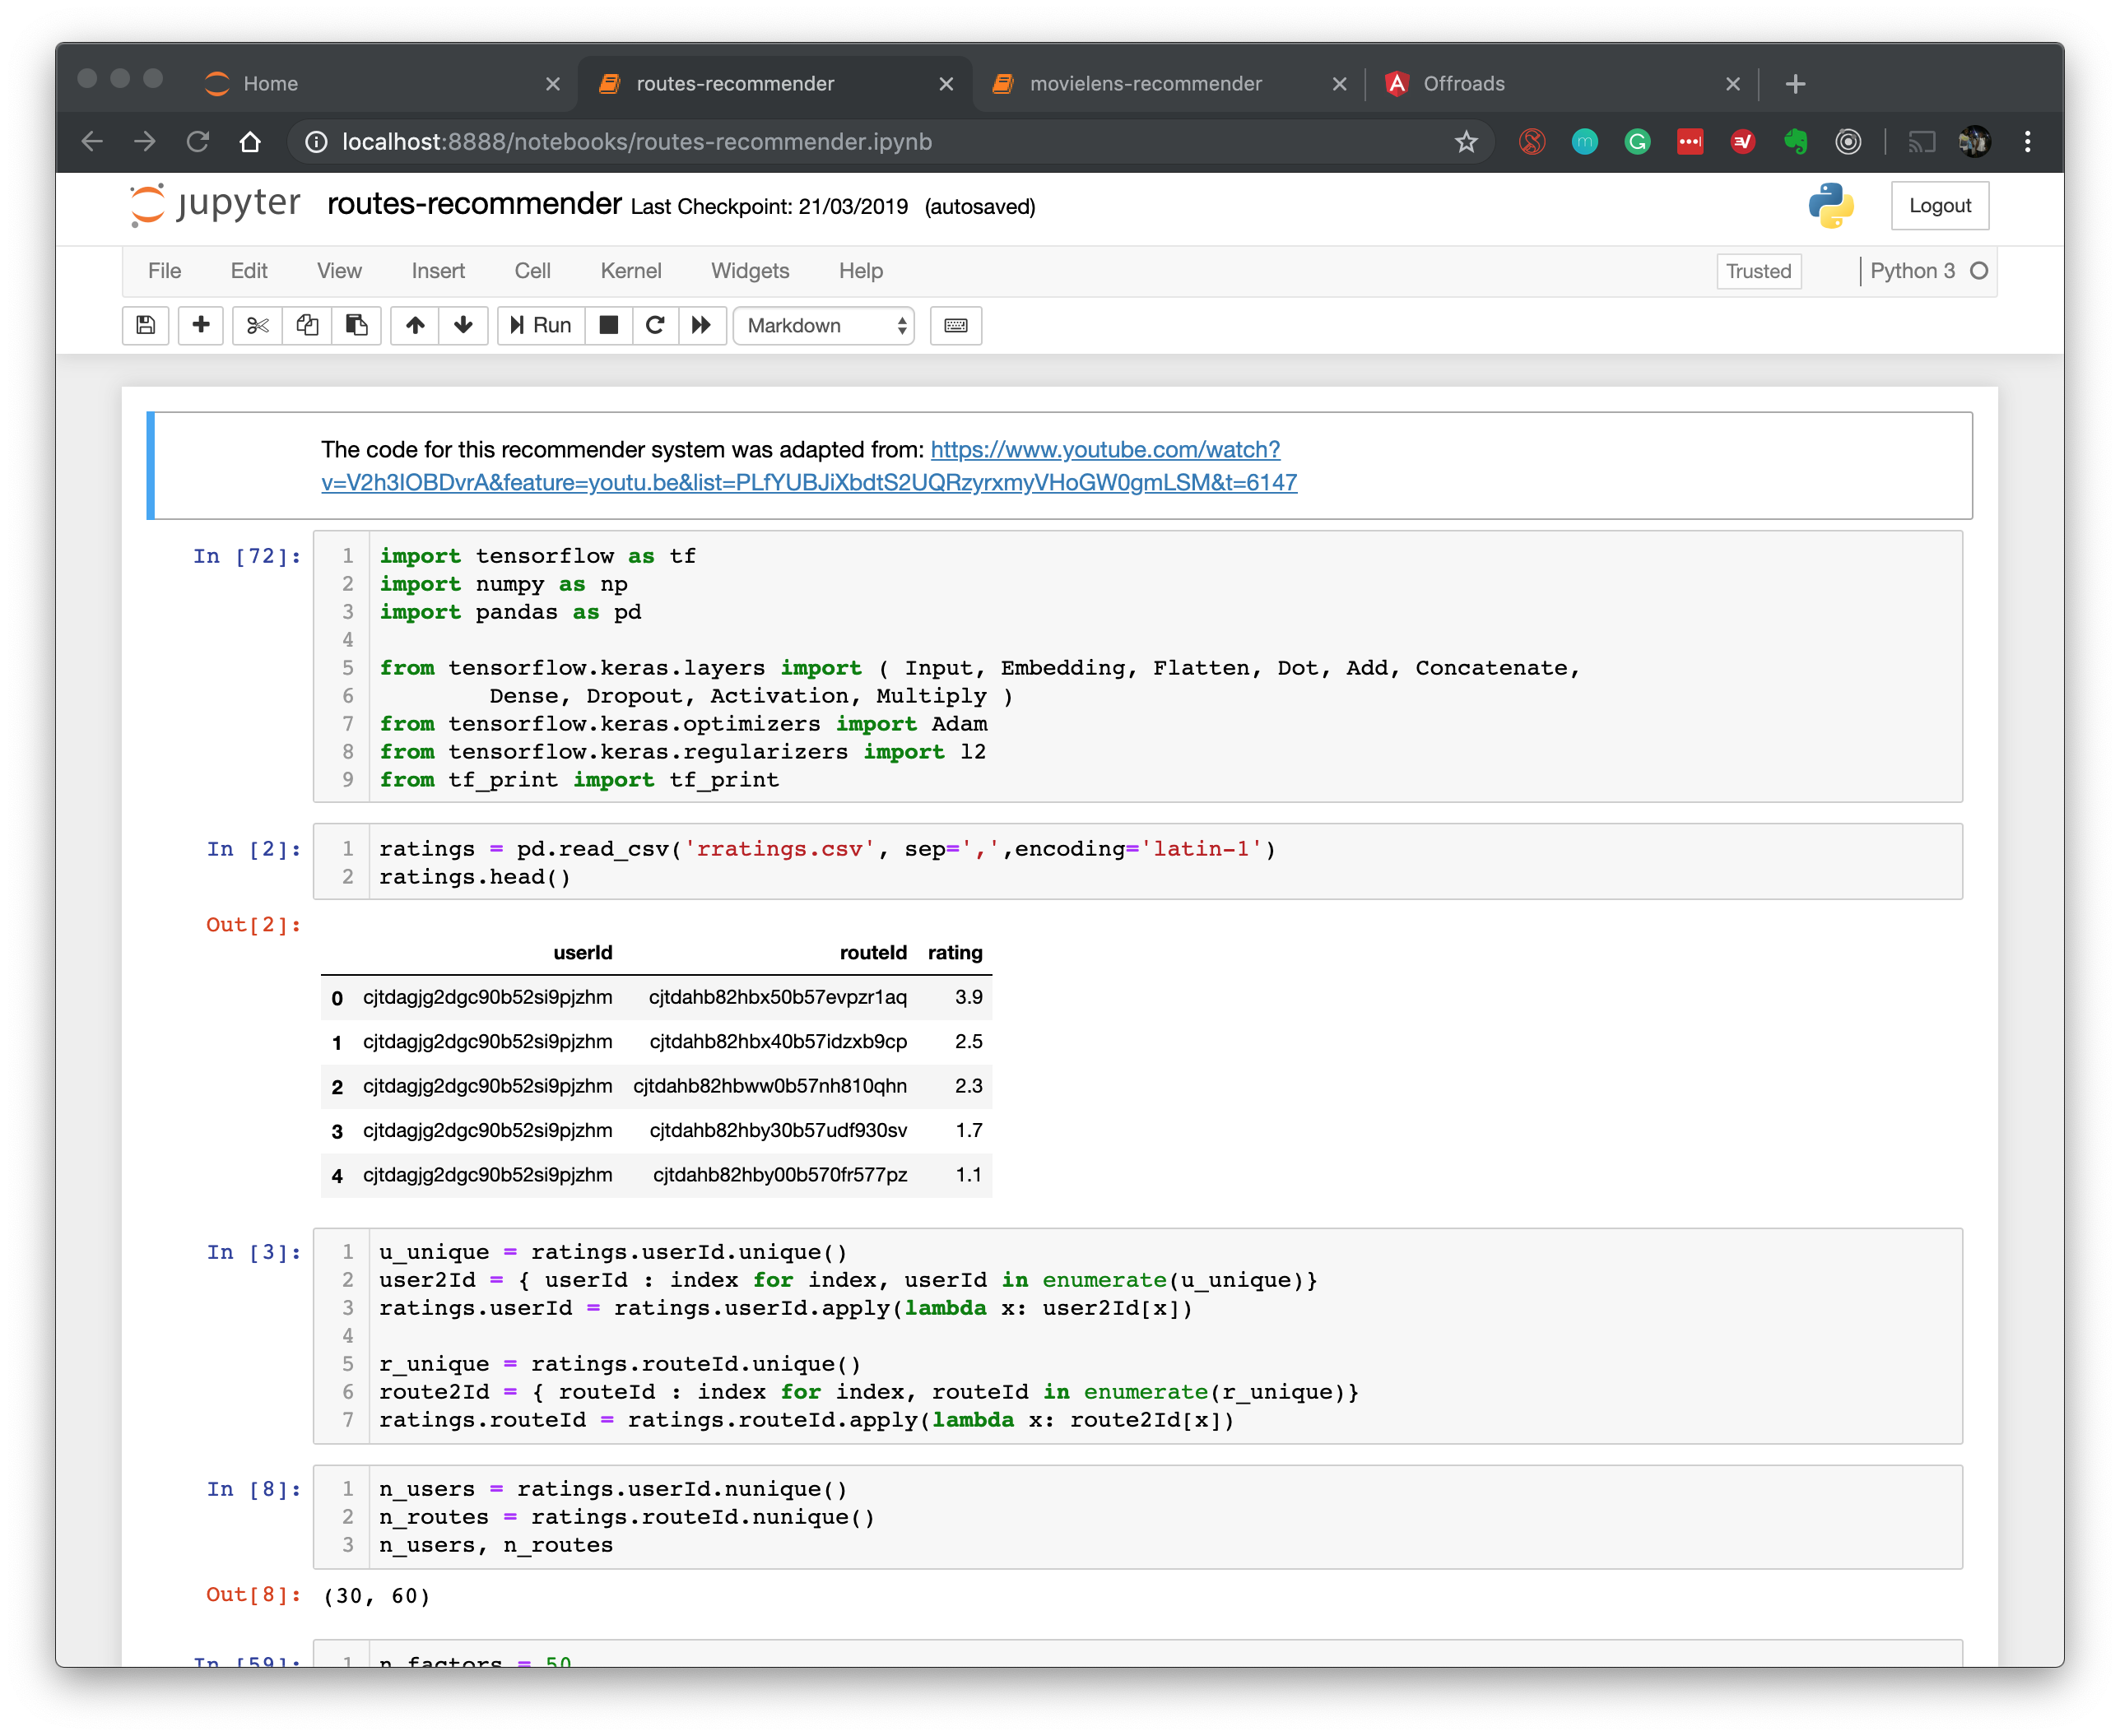
\includegraphics[width=\textwidth]{jupyter-notebook.png}
    \caption{Jupyter Notebook}
    \label{fig:JupyterNotebook}
\end{figure}


\chapter{Evaluation and Testing}
It is important to test the system. Not only manually testing the website, but also empirically testing the efficient of the recommender system. One of the main problems that we have is that we do not have an original dataset to test our system, we discuss ways of overcoming this issue in section \ref{coldStartProble}.
\section{Quality of Recommender systems}
\subsection{Evaluation Metrics}
The quality of recommender systems can evaluated using a variety of different empirical metrics \cite{isinkaye2015recommendation}. We use empirical methods because it gives us a statistical value we can aim to improve. It also gives us a value we can compare against other recommender systems, allowing us to measure against industry standards and benchmarks
\subsection{Extreme Cold Start Problem} \label{coldStartProble}
To test our machine learning model, we would need to have training data to train our model on and then calculate the MSE to know how accurate our model is. However, as this is a completely new system, there is no previous data-set to train the machine learning model on which means that there is no way to test the model. One of the way's to solve this problem is to generate our own dataset.

\subsubsection{Generating Dataset}
Although this will not be an accurate dataset to train our model on, it would help test how good the machine learning model we created is. For the dataset we to need to generate users and routes. For each user and route, we assign 4 attributes: Terrain, Distance, Elevation and Scenery (representing four attributes of a route). For each user, we generate values for these attributes that will correspond with how much each user likes that attribute for a route as shown in table \ref{tab:genUserDataset}. 

The attribute values range from 0 to 9, 0 g extreme dislike and 9 meaning extreme like. Each route will also have values for this attributes which is how much of that attribute that the route has as shown in table \ref{tab:genRouteDataset}.

\begin{table}[ht]
    \centering
    \begin{tabular}{|c|c|c|c|c|}
        \hline
         User ID & Terrain & Distance & Elevation & Scenery  \\
         \hline
         \hline
         0 & 3 & 1 & 3 & 7  \\
         1 & 7 & 8 & 1 & 2 \\
         2 & 8 & 0 & 5 & 2 \\
         4 & 6 & 7 & 7 & 2 \\
         \hline
    \end{tabular}
    \caption{Example of User Data to help generate dataset}
    \label{tab:genUserDataset}
\end{table}

\begin{table}[ht]
    \centering
    \begin{tabular}{|c|c|c|c|c|}
        \hline
         Route ID & Terrain & Distance & Elevation & Scenery  \\
         \hline
         \hline
         0 & 5 & 1 & 3 & 7  \\
         1 & 7 & 5 & 1 & 2 \\
         2 & 8 & 0 & 5 & 8 \\
         4 & 6 & 7 & 7 & 9 \\
         \hline
    \end{tabular}
    \caption{Example of Route Data to help generate dataset}
    \label{tab:genRouteDataset}
\end{table}

We generate 30 users with 5 each from the sub classes in table \ref{tab:attributeSubClasses}. The sub classes are an attempt to represent different types of users and the attribute values are to reflect what they look for int trails. We also generate 60 routes with 10 from each of the sub classes in table \ref{tab:attributeSubClasses}.
\begin{table}[ht]
    \centering
    \begin{tabular}{|c|c|c|c|c|}
        \hline
         Sub-classes & Terrain & Distance & Elevation & Scenery \\
         \hline
         Hardcore & 7 - 9 & 7 - 9 & 7 - 9 & 0 - 9 \\  
         \hline
         Distance & 0 - 3 & 7 - 9 & 0 - 3 & 0 - 3 \\
         \hline
         Visual & 0 - 3 & 0 - 3 & 0 - 3 & 7 - 9 \\
         \hline
         Mountain & 0 - 3 & 0 - 3 & 7 - 9 & 0 - 3 \\
         \hline
         Casual & 0 - 3 & 0 - 3 & 0 - 3 & 0 - 3 \\
         \hline
         Random & 0 - 9 & 0 - 9 & 0 - 9 & 0 - 9 \\
         \hline
    \end{tabular}
    \caption{Caption}
    \label{tab:attributeSubClasses}
\end{table}

Each user runs and rates between 10 and 23 random routes from the generated routes. For each user and the route they run we calculate a \textit{like} value using the attribute values from the user and the route using equation \ref{eqn:Likes}. We then add another probability value that is created using a Gaussian Probability Distribution\cite{simon2007probability} to create and equal probability distribution. This probability value is to add a little bit of randomness to the like value. This represents if for example it was raining when a user runs a route which can affect how they feel about the route compared to normal conditions.

We then use this like value to calculate the rating by using the equation \ref{eqn:RatingCalculation}. We use the Sigmoid function\cite{wiki:SigmoidFunction}, which is a non-linear function\footnote{It's normally used as an activation function in neural networks}, that can map the calculated like value to a value between 0 - 1.

\begin{equation} \label{eqn:Likes}
    \textrm{likes} = \Bigg(\sum_{i=1}^{n=4}abs({u_i}-{r_i})\Bigg) + {p_i}
\end{equation}

\begin{equation} \label{eqn:RatingCalculation}
    \textrm{rating} = \big(\sigma(\textrm{likes}) \times 4\big) + 1
\end{equation}

We then use these generated ratings to help train our machine learning model. With tensor flow we can get our final MSE and root it to get our Root Mean Squared Error (RMSE), the standard for comparing how good the recommender system machine learning models are.

\subsection{Movie Lens Data-set}
Another way to test the system is to use an already existing dataset. One of the benefits of recommender systems is that it can be applied to any generic user-item ratings matrix. Hence although we may not be able to find an already existing user-route ratings matrix, we can use another user-item ratings matrix to test it.

The dataset that I used is a popular dataset of user-movies ratings called the Movie lens Dataset\footnote{https://grouplens.org/datasets/movielens/}. The best thing about using this data set is that there are other online recommender systems that have been tested on this dataset that we can compare our RMSE score against\footnote{https://www.kaggle.com/learn/overview}\footnote{https://www.librec.net/release/v1.3/example.html}.

Create another model that is trained on our movie lens dataset based on the exact same code as the one for our original neural network model.

\section{Manual Testing}
\subsection{GraphQL Dev Tools}
\begin{figure}[ht]
    \centering
    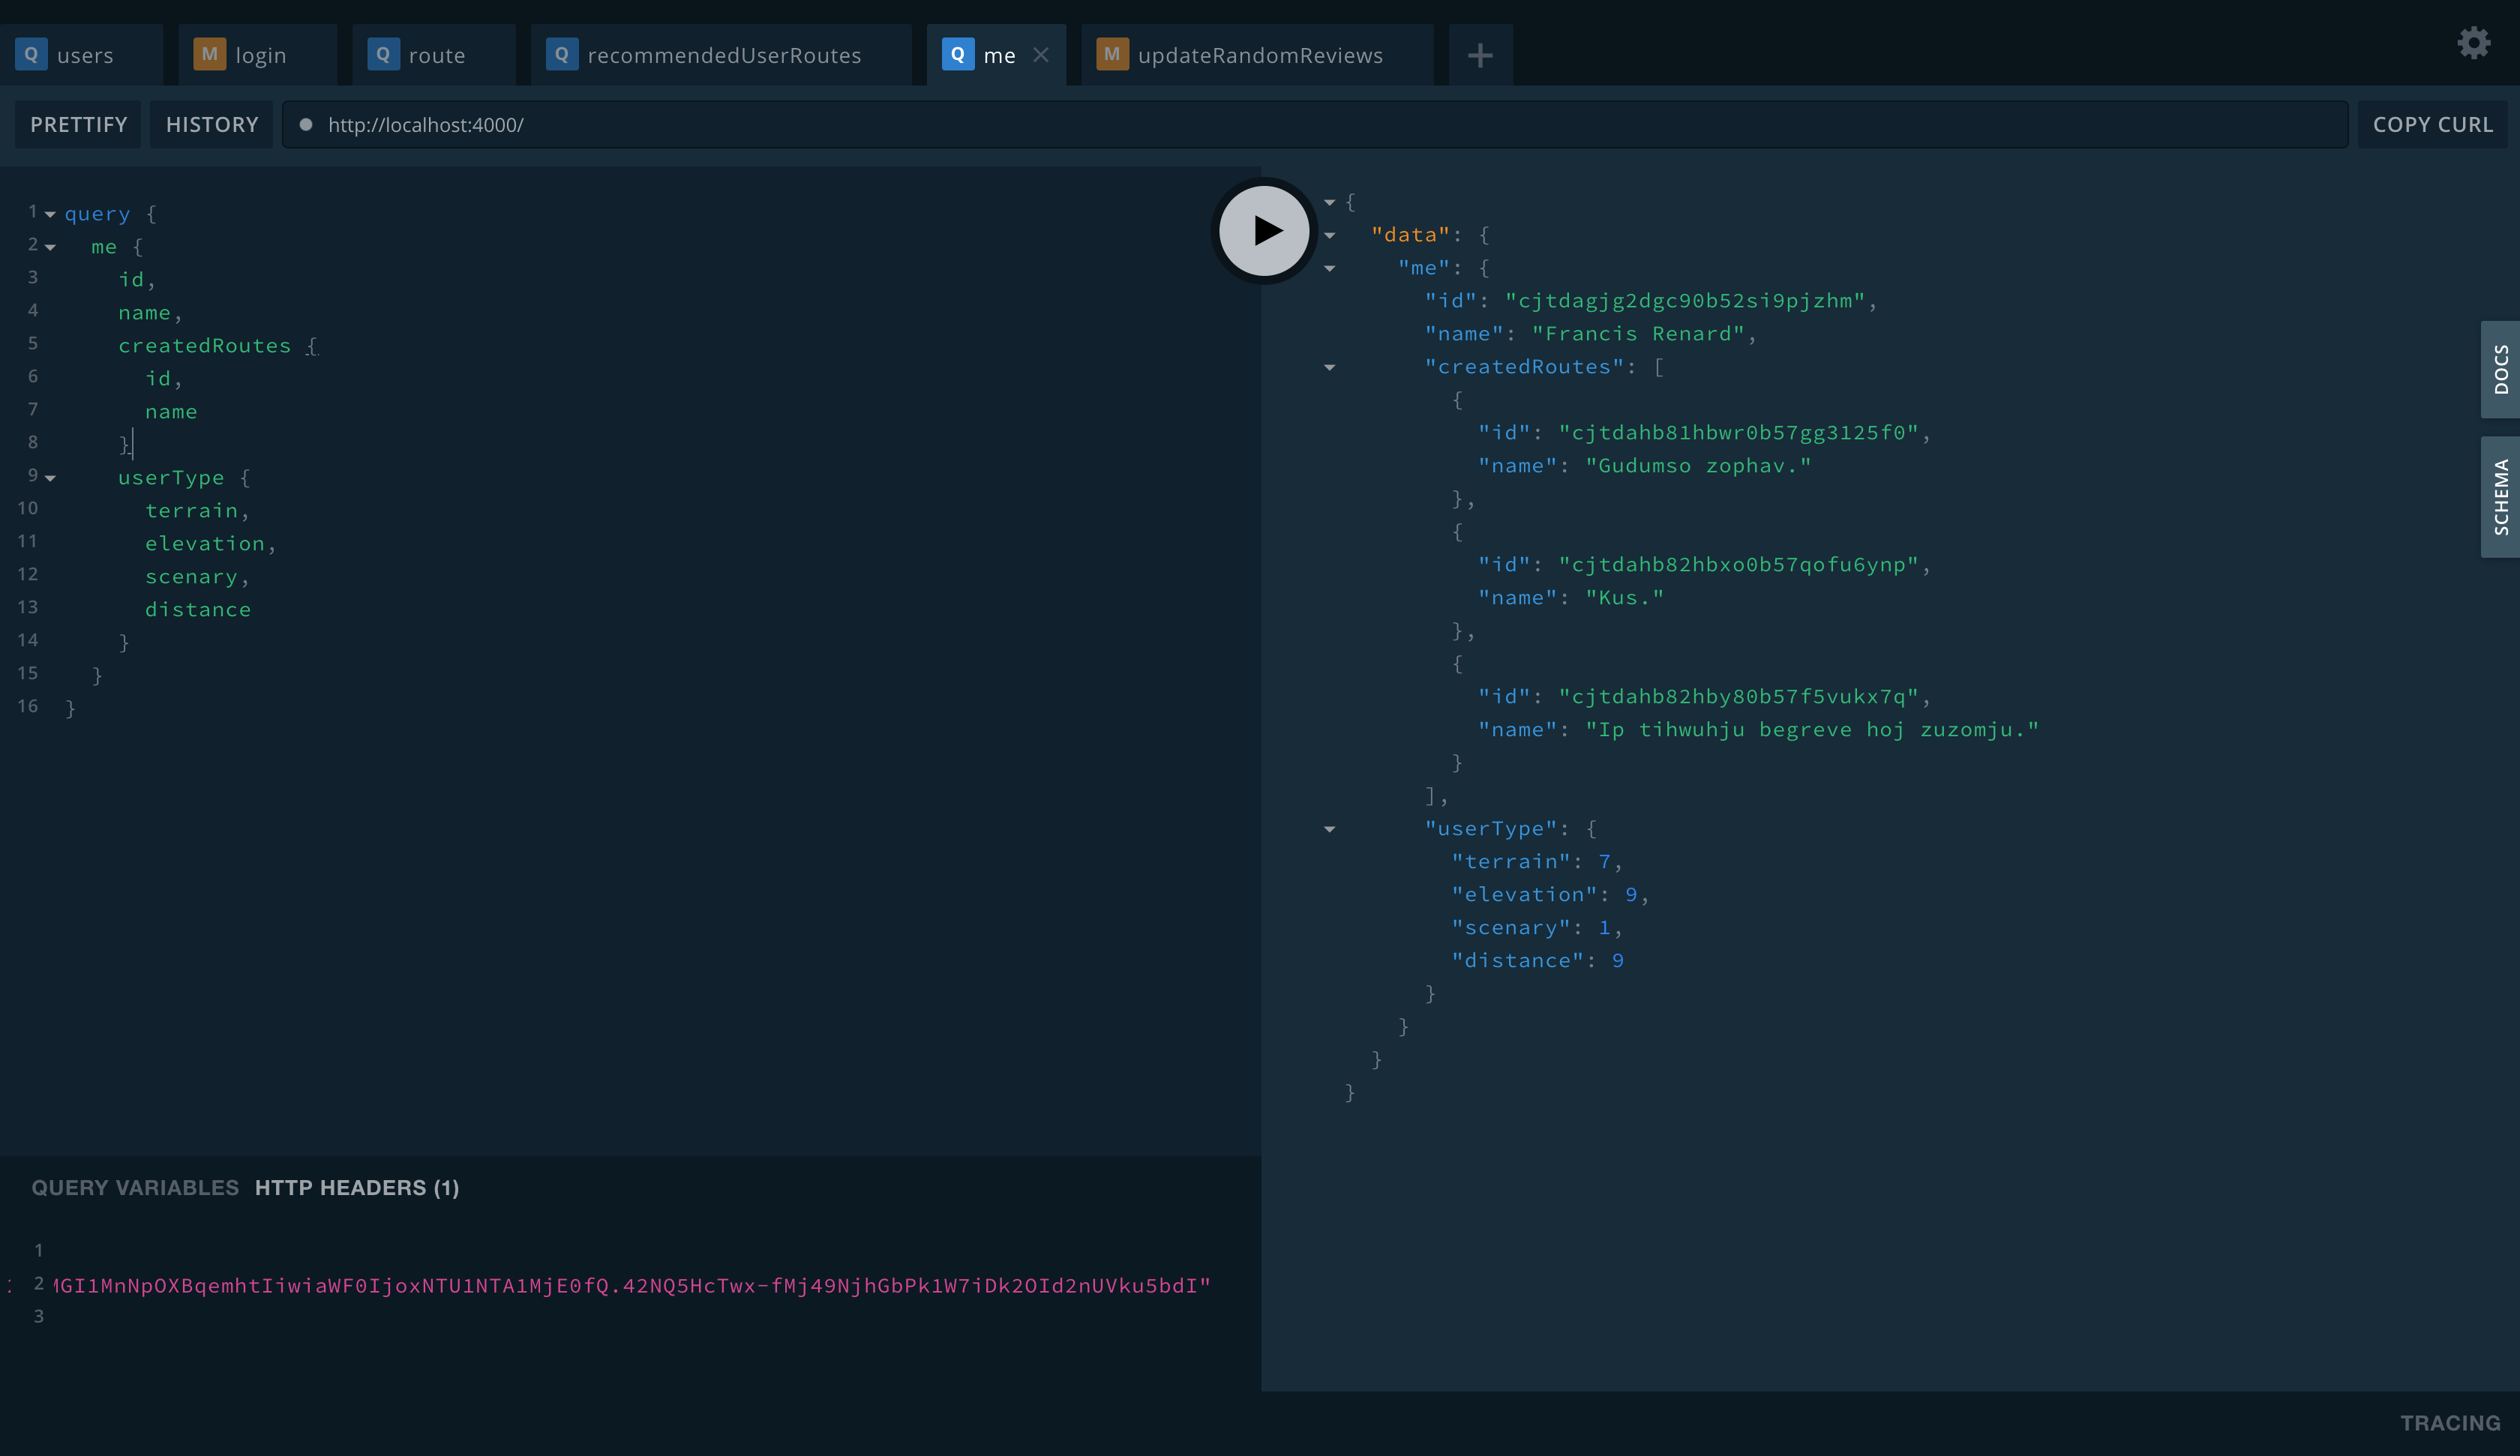
\includegraphics[width=\textwidth]{graphql-dev.png}
    \caption{GraphQl Development Tools}
    \label{fig:graphQLDevTools}
\end{figure}

\section{Unit and Integration Testing}
To test the frontend we follow a standard industry methods of creating both unit tests and integration tests. Angular comes built with the Jasmine Testing framework\footnote{https://jasmine.github.io/}, a javascript behaviour driven framework. Jasmine also use Karma\footnote{https://karma-runner.github.io/latest/index.html}, that allows us to run the tests on the browser.

Angular also provides Protractor\footnote{https://www.protractortest.org/} for end to end testing on the front end
\chapter{Reflections}
\section{Planning and Management}
The project was split into 2 main action areas
\begin{itemize}
    \item The first part was to create the infrastructure of the website. This includes the frontend, backend and the trail interface discussed in the sections above.
    \item The second part was the creation of the recommender system. Including the research into the types of recommender systems that I could use and the technologies.
\end{itemize}

However one of the main problems with this is I greatly underestimated how hard it was building the infrastructure of the website. One of the major factors that slowed me down is learning GraphQL. It is a new technology that I'm not familiar with which made progress with it slow. And as it is quite new, and not used by many, there was no such community to get help from and no real documentation provided to use. 

This meant I was not able to focus alot on researching the recommender system's and could not use Content-based filtering and hybrid recommender systems to improve my overall recommender system.
\section{Future Work}
\subsection{Hybrid Recommender Systems}
One of the problem's we had with this system is there was no extra meta-data on the data for routes given. This prevented us from using content-based filtering. Now although collaborative filtering is a better recommender system than content-based filtering, a much better method would be combining the results from both systems. A hybrid recommender system would be useful to combine and rank the results from both of them to provide between suggestions.

\subsection{Exploring on a Map View}
One of the features that the other trail running websites provide as shown is \autoref{sec:TrailRunningApplications} is presenting the trails on a map view, that show's the location of each trail. This presents a more user friendly way of viewing the trails and also provides extra information of the location of where the trails are.

\subsection{Deploying the Website}
An important part of building any application is the method of deployment. I would have used one of the many online cloud services, preferably Amazon Web Services (AWS), to deploy the website. One of the mahor things of using this is that it allow's you to easily build scalable web applications. They also take away the complexity of dealing with hard ware issues. And it would provide extra resources needed, for example, machine learning specific architecture to improve the machine learning process.

\subsection{CI \& CD pipelines}
During development, I used alot of development tools. One strategy I could use to make both debugging and deployment easy is to use Continous Integration and Continous Deployment. This is very important for improving real life applications as it eleviates the problems that come with testing by adding automated testing and ensuring the main version of the application is not broken. It also simplifies the deployment of applications

\subsection{Mobile Application}
One of the problems with building a website solution is that it's not a very mobile solution. It's not easy to allow users to live record a trail as they run it, or their live data as they run an already ran trail to help in comparison. 

A better way for deliver this solution is to use a mobile application. However with a mobile application there's also the problem of developing for multiple Operating Systems, namely IOS and Android.

So we could use a hybrid framework to develop for both of these interfaces. I believe this would be a better solution than just developing a responsive website as it would have a more native feel. And it would have the benefit of not having to develop and maintain different projects for the same application.
\chapter{Conclusion}


\printglossary
\printglossary[type=\acronymtype]

\printbibliography[heading=bibintoc]

\begin{appendices}
    \chapter{Mapping data returned} \label{appendix:mapDataReturned}

\section*{Mapbox Directions Result} \label{appSec:mapboxDirections}
\inputminted[frame=lines,framesep=2mm,baselinestretch=1.2,fontsize=\footnotesize]{json}{listings/mapbox-directions.json}
\captionof{listing}{Example of Directions returned from mapbox directions API}

\section*{Google Maps Elevation Results} \label{appSec:googleElevation}
\inputminted[frame=lines,framesep=2mm,baselinestretch=1.2,fontsize=\footnotesize]{json}{listings/google-elevation.json}
\captionof{listing}{Example of Google's elevation service data returned}
    \chapter{Server GraphQL Schema} \label{app:graphqlSchema}
\end{appendices}
\end{document}
